\documentclass{beamer}

\usepackage{tabularx,ragged2e,booktabs,caption}
\usepackage{multirow}
\usepackage{xcolor}
\usepackage{colortbl}
\usepackage{multicol}
\usepackage{fullpage,graphicx}

\mode<presentation> {
	\usetheme{Madrid}
	%\usetheme{Malmoe}
	%\usetheme{Marburg}
	%\usetheme{Montpellier}
	%\usetheme{PaloAlto}
	%\usetheme{Pittsburgh}
	%\usetheme{Rochester}
	%\usetheme{Singapore}
	%\usetheme{Szeged}
	%\usetheme{Warsaw}

	% As well as themes, the Beamer class has a number of color themes
	% for any slide theme. Uncomment each of these in turn to see how it
	% changes the colors of your current slide theme.

	%\usecolortheme{albatross}
	%\usecolortheme{beaver}
	%\usecolortheme{beetle}
	%\usecolortheme{crane}
	%\usecolortheme{dolphin}
	%\usecolortheme{dove}
	%\usecolortheme{fly}
	%\usecolortheme{lily}
	%\usecolortheme{orchid}
	%\usecolortheme{rose}
	%\usecolortheme{seagull}
	%\usecolortheme{seahorse}
	%\usecolortheme{whale}
	%\usecolortheme{wolverine}

	%\setbeamertemplate{footline} % To remove the footer line in all slides uncomment this line
	%\setbeamertemplate{footline}[page number] % To replace the footer line in all slides with a simple slide count uncomment this line

	%\setbeamertemplate{navigation symbols}{} % To remove the navigation symbols from the bottom of all slides uncomment this line
}

\usepackage{graphicx} % Allows including images
\usepackage{booktabs} % Allows the use of \toprule, \midrule and \bottomrule in tables

\setbeamercovered{invisible}
\setbeamercovered{again covered={\opaqueness<1->{30}}}

\newenvironment{centerverbatim}{%
	\par
	\centering
	\varwidth{\linewidth}%
	\verbatim
}{%
	\endverbatim
	\endvarwidth
	\par
}

% PYTHON
% Default fixed font does not support bold face
%\DeclareFixedFont{\ttb}{T1}{txtt}{bx}{n}{12} % for bold
%\DeclareFixedFont{\ttm}{T1}{txtt}{m}{n}{12}  % for normal
%
% Custom colors
%\usepackage{color}
%\definecolor{deepblue}{rgb}{0,0,0.5}
%\definecolor{deepred}{rgb}{0.6,0,0}
%\definecolor{deepgreen}{rgb}{0,0.5,0}
%
% Python style for highlighting
%\newcommand\pythonstyle{\lstset{
%		language=Python,
%		morekeywords={self},              % Add keywords here
%		keywordstyle=\footnotesize\color{deepblue},
%		emph={MyClass,__init__},          % Custom highlighting
%		emphstyle=\footnotesize\color{deepred},    % Custom highlighting style
%		stringstyle=\color{deepgreen},
%		frame=tb,                         % Any extra options here
%		showstringspaces=false,
%		basicstyle=\footnotesize,
%		numbers=left,
%		stepnumber=1
%}}
%
% Python environment
%\lstnewenvironment{python}[1][]
%{
%	\pythonstyle
%	\lstset{#1}
%}
%{}
%
% Python for external files
%\newcommand\pythonexternal[2][]{{
%		\pythonstyle
%		\lstinputlisting[#1]{#2}}}
%
% Python for inline
%\newcommand\pythoninline[1]{{\pythonstyle\lstinline!#1!}}

\makeatletter
\newcounter{ftitle}
\long\def\beamer@@frametitle[#1]#2{%
	\beamer@ifempty{#2}{}{%
		\gdef\insertframetitle{{#2\ifnum\beamer@autobreakcount>0\relax{}\space\usebeamertemplate*{frametitle continuation}\fi}}%
		\gdef\beamer@frametitle{#2}%
		\stepcounter{ftitle}
		\expandafter\gdef\csname Frametitle\romannumeral\theftitle\endcsname{#2}
		\gdef\beamer@shortframetitle{#1}%
	}%
}
\makeatother

%%%%%%%%%%%%%%%%%%%%%

%%%%%% CONTENT %%%%%%%%%

%%%%%%%%%%%%%%%%%%%%%

\title[]{Desarrollo de una medida de similaridad para Sistemas de Recomendación en sitios de Community Question Answering. Análisis desde un enfoque Big Data y usando un método de ensamble de clustering} % The short title appears at the bottom of every slide, the full title is only on the title page

\author{Ing. Federico Tesone} % Your name
\institute[UTN] % Your institution as it will appear on the bottom of every slide, may be shorthand to save space
{
	Universidad Tecnológica Nacional (FRR) \\ % Your institution for the title page
	\medskip
	% textit{john@smith.com} % Your email address
}
\date{Fecha pendiente} % Date, can be changed to a custom date
\setcounter{tocdepth}{1}

\begin{document}

	\begin{frame}
		\titlepage
	\end{frame}

	\begin{frame}
	Aca va el jurado y eso

		\begin{figure}
			\includegraphics[width=0.1\linewidth]{../imagenes/portada/logoUTN.png}
		\end{figure}
	\end{frame}

	\begin{frame}[allowframebreaks]
		\frametitle{Tabla de contenidos}
		\scriptsize
		\tableofcontents
	\end{frame}

	\section{Introducción}

\subsection{Área temática}
\begin{frame}{Área temática}
	Este trabajo se basa en 5 pilares teóricos:
	\medskip
	\begin{itemize}[<*>]
		\item Sistemas de Recomendación.
		\item Sitios de Community Question Answering (CQA).
		\item Medidas de similaridad.
		\item Ensamble de Clustering.
		\item Big Data.
	\end{itemize}
\end{frame}

\begin{frame}{Área temática II}
	\textbf{Area temática}
	\medskip
	\begin{itemize}
		\item Miles de nuevas preguntas son formuladas diariamente en sitios de CQA como Yahoo! Answers, Stackexchange, Stackoverflow, o Quora.
		\item Muchas de las preguntas no están respondidas correctamente o no tienen respuestas.
		\begin{itemize}[<*>]
			\item Pequeño número de expertos entre la gran población de usuarios.
			\item La pregunta es difícil de ubicar dentro del sitio.
			\item Respuestas maliciosas.
		\end{itemize}
		\item Es de interés buscar si esa misma pregunta ha sido formulada por otro usuario previamente, y que tenga la respuesta buscada.
		\item Preguntas que poseen la misma respuestas están formuladas de forma diferente en el sentido léxico. \\
		\begin{center}
			\begin{footnotesize}
				\textit{¿Cómo elijo una revista para publicar mi artículo?} y \textit{¿Dónde publico mi artículo?}
			\end{footnotesize}
		\end{center}
	\end{itemize}
 \end{frame}

\begin{frame}{Área temática III}
	\textbf{Area temática (cont.)}
	\medskip
	\begin{itemize}
		\item Es necesaria una medida de similaridad que tenga en cuenta características léxicas y semánticas.
		\item La tarea de recomendar preguntas similares en sitios de CQA puede ser llevada a cabo por un RS.
		\item Se diseñó e implementó una arquitectura Big Data para crear una medida de similaridad que alimente a un RS para sitios de CQA.
	\end{itemize}
\end{frame}

\subsection{Tema específico}
\begin{frame}[allowframebreaks]{Tema específico}
	Pipeline para un RS basado en contenido de CQA y en una nueva medida de similaridad.
	\medskip
	\begin{figure}
		\centering
		\includegraphics[width=0.7\linewidth]{../5_introduccion/imagenes/pipeline}
		\label{fig:pipeline}

		\bigskip

		Este trabajo se enfoca en el \textbf{Paso 2} del pipeline.

		\framebreak

		Considerando el conjunto completo de datos Quora (\(404301\) pares de preguntas, es decir, \(808602\) preguntas totales), deberíamos realizar:

		\bigskip $\frac{n(n+1)}{2} = 326919001503$ calculos de distancias, donde $n = 808602$

		\bigskip
		\bigskip

		Esta situación plantea la necesidad de considerar una arquitectura Big Data.
	\end{figure}
\end{frame}

\subsection{Objetivo general}
\begin{frame}{Objetivo general}
	\begin{tcolorbox}[colback=blue!5,colframe=blue!40!black,title=Objetivo general]
	El presente trabajo de investigación tiene como objetivo construir una \textbf{arquitectura Big Data} que incluye la posibilidad de ser aplicada a grandes conjuntos de datos en el ámbito de \textbf{CQA} y, a partir de esta arquitectura, implementar, evaluar y realizar un \textbf{análisis comparativo con el estado del arte de una nueva medida de similaridad entre textos} que pueda ser utilizada en \textbf{Sistemas de Recomendación}.
	\end{tcolorbox}
\end{frame}

\subsection{Objetivos específicos}
\begin{frame}{Objetivos específicos}
	\begin{tcolorbox}[colback=blue!5,colframe=blue!40!black,title=Objetivos específicos]
		\begin{footnotesize}
			\begin{itemize} [<+>]
				\item Diseñar y desarrollar una \textbf{arquitectura Big Data} para cálculo de similaridad en grandes volúmenes de datos.
				\item Identificar \textbf{medidas de similaridad de texto} existentes y un método efectivo de aplicación de las mismas en grandes volúmenes de datos.
				\item \textbf{Proponer una nueva medida} que permita integrar las medidas de similaridad del estado del arte mediante una arquitectura de software basada en Big Data.
				\item \textbf{Evaluar el comportamiento} de una medida de similaridad de texto del estado del arte respecto al manejo del volumen, variedad, velocidad y veracidad inherentes a grandes volúmenes de datos.
				\item \textbf{Brindar conclusiones, pautas y recomendaciones} para trabajar con medidas de comparación de textos en grandes volúmenes de datos en sitios de CQA utilizando arquitecturas basadas en Big Data.
			\end{itemize}
		\end{footnotesize}
	\end{tcolorbox}
\end{frame}
	\newpage \section{Fundamentación}\label{ch:fundamentacion}
\subsection{Estado del arte}
\subsubsection{Sitios de CQA}
\noindent Los servicios de Community Question Answering CQA, son un tipo especial de servicios \textit{Question Answering} (QA), los cuales permiten a los usuarios registrados responder a preguntas formuladas por otras personas. Los mismos atrajeron a un número creciente de usuarios en los últimos años \citep{li2010routing}. Una pregunta formulada en Quora, y respondida por su fundador y CEO, Adam D\textsc{\char13}Angelo, revela que el sitio recibe más de 200 millones de visitantes únicos mensualmente (información actualizada a Junio de 2017), lo que denota la popularidad de este tipo de portales\footnote{Pregunta formulada en el sitio Quora \textit{``How many people use Quora?''}: \url{https://www.quora.com/How-many-people-use-Quora-7}. Último acceso Agosto 2018.}. Desde la creación de este tipo de servicios, se han aplicado diferentes técnicas de software para que los usuarios encuentren respuestas a sus preguntas en el menor tiempo posible y aprovechar al máximo el valor de las bases de conocimiento, por ejemplo, un framework para predecir la calidad de las respuestas con características no textuales \citep{jeon2006framework}, incorporar información de legibilidad en el proceso de recomendación \citep{anuyah2017can}, encontrar a los expertos apropiados \citep{li2010routing} o recomendar la mejor respuesta a una pregunta dada, entre otros. Sin embargo, el mecanismo existente en el cual se responden las preguntas en los sitios de CQA todavía no alcanza a satisfacer las expectativas de los usuarios por varias razones: 
\begin{inparaenum}[(1)]
	\item baja probabilidad de encontrar al experto: una nueva pregunta, en muchos casos, puede no encontrar a la persona con la habilidad de responderla de manera correcta, resultando en respuestas tardías y que distan de ser óptimas; 
	\item respuestas de baja calidad: los sitios de CQA suelen contener respuestas de baja calidad, maliciosas y spam. Estas suelen recibir baja calificación de los miembros de la comunidad; \item preguntas archivadas y poco consultadas: muchas preguntas de los usuarios son similares. Antes de formular una pregunta, un usuario podría beneficiarse de buscar ya formuladas, y por consiguiente, sus respuestas \citep{yang2013cqarank}.
\end{inparaenum}

\subsubsection{Sistemas de recomendación}
\noindent Es muy frecuente tener que tomar decisiones sin la suficiente experiencia personal sobre las alternativas disponibles. En la vida cotidiana, confiamos en recomendaciones de otras personas ya sea de boca en boca o cartas de recomendación, reseñas de libros y películas o encuestas generales. Los sistemas de recomendación asisten este proceso natural en el ámbito de los sistemas de información \citep{resnick1997recommender}. El primer RS, \textit{Tapestry} \citep{goldberg1992using}, fue un sistema experimental de correo electrónico destinado a resolver el problema de manejar grandes cantidades de emails filtrando según cuán interesantes son los documentos, utilizando un enfoque basado en el contenido de los mismos y también filtros colaborativos, lo que después se denominaría RS no personalizados y personalizados por \citeauthor{ricci2011introduction} en el año \citeyear{ricci2011introduction}. Se ha trabajado mucho en mejorar y desarrollar nuevos enfoques con respecto a RS en los últimos años, y el interés en esta área sigue vigente debido a la abundancia de aplicaciones prácticas en las cuales es necesario ayudar a los usuarios a lidiar con la sobrecarga de información\footnote{El concepto de sobrecarga de información, del inglés \textit{information overload}, hace referencia a cuando los usuarios reciben demasiada información, por lo cual, la precisión en sus decisiones empieza a decrecer \citep{eppler2004concept}.} y proveer recomendaciones personalizadas, contenidos y servicios. Sin embargo, a pesar de todos estos avances, la generación actual de RS todavía requiere mejoras para que los métodos de recomendación sean más efectivos y aplicables a una gama más amplia de sistemas y/o sitios. Aunque las raíces de los RS se remontan a trabajos en ciencia cognitiva \citep{rich1979user}, teoría de aproximación \citep{powell1981approximation}, recuperación de información \citep{salton1989automatic}, ciencias de las predicciones \citep{armstrong2001principles}, ciencias de la gestión \citep{murthi2003role} y también al modelado de la elección de consumidor en marketing \citep{lilien1992marketing}, los RS recién surgen como un área de investigación independiente en la década de 1990, cuando los investigadores comenzaron a centrarse en problemas de recomendación que se basan específicamente en calificaciones \citep{adomavicius2005toward}. En su formulación más común, el problema de recomendación se reduce a estimar calificaciones para los ítems que no han sido vistos por un usuario.

\subsubsection{Big Data}
\noindent Al igual que todos los términos que surgen a partir de avances tecnológicos, no existe un consenso claro de cómo definir \textit{Big Data}. \cite{manyika2011big} definen este concepto como los conjuntos de datos cuyo tamaño está más allá de la habilidad de las herramientas software de base de datos para capturar, almacenar, gestionar y analizar. Nótese que esta definición es agnóstica del tamaño del conjunto de datos, y no define un tamaño mínimo del mismo, sino que, asume que la tecnología avanza constantemente como así también las herramientas, por lo cual, la definición se “mueve” con el tiempo. Por otro lado, también es interesante tomar otra arista en la definición de este concepto. La consultora Gartner en su sitio web\footnote{Concepto de Big Data en el glosario de Gartner: \url{https://www.gartner.com/it-glossary/big-data}. Último acceso Agosto 2018.} lo define como “Big Data son activos de información caracterizados por su alto volumen, velocidad y variedad que demandan formas innovadoras y rentables de procesamiento de información para mejorar la compresión y la toma de decisiones”, haciendo énfasis en la multiplicidad de características de Big Data. 

\bigskip El comienzo de sobrecarga de información, recientemente mencionado, data del año 1880, cuando el censo de los Estados Unidos tarda 8 años en tabularse. Ante esta situación Herman Hollerith inventó la máquina tabuladora eléctrica basada en tarjetas perforadas\footnote{Herman Hollerith, US Census Boureau: \url{https://www.census.gov/history/www/census_then_now/notable_alumni/herman_hollerith.html}. Último acceso Agosto 2018.}. El censo en 1890 fue un éxito rotundo e, incluso, la máquina que él diseñó fue  utilizada para los censos de Canadá, Noruega y Austria al año siguiente.

\bigskip En el año 1941, los científicos empiezan a utilizar el término “explosión de la información”, que fuera  citado en el periódico The Lawton Constitution\footnote{The Lawton Constitution: \url{http://www.swoknews.com/}. Último acceso Agosto 2018.}, haciendo alusión a la dificultad de administrar toda la información disponible. Gradualmente, se identificaron avances concretos en materia de procesamiento de datos y criptografía, motivados particularmente por los sucesos bélicos de la época. Un ejemplo es el dispositivo llamado Colossus \citep{copeland2004colossus} que buscaba e interceptaba mensajes a una tasa de miles de caracteres por segundo. Unos años más tarde, en 1951 el concepto de \textit{memoria virtual} es introducido por el físico alemán Fritz-Rudolf Güntsch, como una idea que trataba el almacenamiento finito como infinito.

\bigskip A partir de la década del 80', los avances tecnológicos, especialmente en sistemas MRP (planificación de recursos de fabricación), permitieron nuevas formas de organizar, almacenar y generar datos. En este sentido, IBM se destaca y define una arquitectura para los informes y análisis de negocio (EBIS)\footnote{Acrónimo para EMEA (Europe, Middle East and Africa) Business Information System.}, que se convierte en la base del almacenamiento de datos en forma centralizada para usuarios finales \citep{devlin1988architecture}; es decir, el \textit{data warehousing}. Hacia finales de los 80’, Tim Berners-Lee, inventa la \textit{World Wide Web} \citep{berners1992world}. Invento que implicaría el impacto más grande hasta la actualidad con respecto a la generación, identificación, almacenamiento y análisis de grandes volúmenes de datos de diversa naturaleza.

\bigskip El inicio de los años 90’ marcan un antes y un después en lo relativo al tratamiento y almacenamiento de datos. El crecimiento tecnológico fue explosivo, tal es así que el almacenamiento digital empieza a ser más conveniente y rentable que el papel para almacenar datos \citep{morris2003evolution}. Es en 1990 cuando surgen las plataformas de \textit{Business Intelligence} (BI) y los rediseños de software al estilo \textit{Enterprise Resource Planning} (ERP). En este contexto, \cite{cox1997application} afirman que el crecimiento de la cantidad de datos que debe manejar un sistema de información empieza a ser un problema en materia de almacenamiento y visualización de los datos, situación que denominaron como “el problema del Big Data”. Así, 1997 es un año clave, en el que se realizan un gran porcentaje de estudios y publicaciones que se enfocan en averiguar cuánta información hay disponible a nivel mundial y su crecimiento\footnote{Michael Lesk publica “How much information is there in the world?” (1997): \url{http://www.lesk.com/mlesk/ksg97/ksg.html}. Último acceso Agosto 2018.}, y, en consecuencia, se estima que el crecimiento de Internet es aproximadamente del 100\% anual y que superaría el tráfico de voz para el año 2002 \citep{coffman1998size}.

\bigskip En el año 2001, se introduce el concepto de \textit{las 3 V’s: Volumen, Velocidad y Variabilidad de los datos} \citep{laney20013d} fundantes sobre la temática y que sería mundialmente aceptado una década más tarde. Por otro lado, también, en 2001 aparece el concepto de \textit{Software como un Servicio} (SaaS) \citep{hoch2001software}, un modelo disruptivo de servicios centralizados y acceso a los mismos mediante clientes finos (típicamente exploradores web), dando la posibilidad del escalamiento horizontal de sistemas de información y la generación de estándares de comunicación. Esta situación provocó que empresas como Oracle\footnote{Oracle: \url{https://www.oracle.com}. Último acceso Agosto 2018.}, SAP\footnote{SAP: \url{https://www.sap.com}. Último acceso Agosto 2018.}, y Peoplesoft\footnote{Peoplesoft: adquirida por Oracle en Enero de 2005.} empiecen a centrarse en el uso de servicios web, permitiendo así la generación de datos en forma masiva por usuarios finales. Así, en 2006, nace Apache Hadoop\footnote{Apache Hadoop: \url{http://hadoop.apache.org/}. Último acceso Agosto 2018.}, una solución de código abierto que permite el procesamiento en paralelo y distribuido de enormes cantidades de datos en forma escalable. Posteriormente, en 2008, se empieza a pensar al Big Data como la mayor innovación en informática en la última década, ya que ha transformado la forma en que los motores de búsqueda acceden a la información, las actividades de las compañías, las investigaciones científicas, la medicina, y las operaciones de defensa e inteligencia de los países, entre otras tantas actividades. Más aún, se ha comenzado a ver su potencial para recopilar y organizar datos en todos los ámbitos de la vida cotidiana \citep{bryant2008big}, tales como redes sociales, estadísticas deportivas o avances médicos y genéticos.

\subsection{La propuesta}
\noindent La calidad de un RS tiene una relación directa con los datos de entrada que se han generado para alimentarlo. Con el fin de generar una entrada basada en medidas de similaridad, es necesaria la comparación de preguntas formuladas en sitios de CQA usando técnicas de análisis de texto.
Un problema importante inherente al análisis de texto, con el fin de cuantificar relaciones entre distintos fragmentos o documentos, es encontrar la medida apropiada de representación. Algunas medidas de similaridad resultantes de algoritmos de recomendación en análisis de texto, son obtenidas mediante algoritmos puramente sintácticos, léxicos, tales como: \textit{Term Frequency} \citep{salton5mcgill}, \textit{Term Frequency/Inverse Document Frequency} \citep{baeza1999modern}, basados en ventanas como \textit{FastText} \citep{joulin2016fasttext} o \textit{Word2Vec} \citep{mikolov2013efficient}, o semánticos, como \textit{Semantic Distance} \citep{li2006sentence}. Los algoritmos puramente sintácticos como Term Frequency y Term Frequency/Inverse Document Frequency tienen conocidos problemas, tales como ser invariantes respecto al orden de las palabras o ser sensibles a stopwords, por lo cual, necesitan un gran trabajo de pre-procesamiento. FastText y Word2Vec están fuertemente afectados en el orden en el cual aparecen las palabras. Adicionalmente, ninguna de estas técnicas tiene en cuenta la semántica de las palabras y sus relaciones, como si lo hace Semantic Distance. Sin embargo, esta última técnica, según el trabajo tomado como estado del arte, tampoco alcanza medidas de rendimiento apropiadas para un RS en un sitio de CQA.

\bigskip Resultados experimentales de medidas de rendimiento obtenidas en el trabajo que se toma como punto de partida de esta tesis, arrojan entre un 66\% y un 68\% de precisión y entre un 32\% y un 33.5\% de error usando cada uno de los algoritmos de recomendación descritos anteriormente. Estos valores son considerados prometedores, ya que las medidas de rendimiento son consistentes en todos los algoritmos seleccionados, lo que denota que la complejidad inherente del conjunto de datos no afecta significativamente la performance de cada uno de ellos. Además, los resultados de prueba no varían significativamente con respecto a los resultados de validación. Dicho esto, la motivación de este trabajo de tesis, así como el de las futuras líneas de investigación, es la creación de una medida de similaridad de texto novedosa que sirva como entrada para un RS aplicable a sitios de CQA. Para tal fin, se crearán matrices de distancias, usando cada una de las preguntas del conjunto de datos en estudio, para luego combinarlas usando métodos de ensamble de clustering, ya que, como existen cientos algoritmos de clustering, es difícil identificar un solo algoritmo que pueda manejar todos los tipos de forma y tamaños de cluster, e incluso, decidir qué algoritmo sería el mejor para un conjunto de datos en particular. \cite{fred2005combining} introducen el concepto de clustering de acumulación de evidencias, que mapea las particiones de datos individuales en un ensamble de clustering dentro de una nueva medida de similaridad entre patrones, sumarizando la estructura entre-patrón percibido de esos clusters. La partición de datos final es obtenida aplicando el método \textit{single-linkage} a la nueva matriz de similaridad. El resultado de este método muestra que, la combinación de algoritmos de clustering “débiles” como el \textit{k-means}, pueden conducir a la identificación de clusters subyacentes verdaderos con formas, tamaños y densidades arbitrarias. Por lo cual, teniendo en cuenta diferentes particiones creadas con el método de ensamble desde los mismos datos originales, objetos de textos similares probablemente pertenecerán al mismo cluster.

\bigskip El desarrollo de matrices de similaridad para la aplicación del EAC que se utilizarán como entrada de RS, claramente implica manipular un gran volumen de datos complejos y realizar un elevado número de cálculos en tiempo real, ya que nos estamos refiriendo a conjuntos de datos cuyo tamaño supera la capacidad de las herramientas tradicionales de bases de datos de recopilar, almacenar, gestionar y analizar la información \citep{de2016mineria}. Esto implica, en principio, considerar una \textit{matriz de co-asociación} entre elementos realizando varias series de corridas y aplicación de clustering. Cada una de esas series es basada en una de las medidas de similaridad. El resultado será un un valor adimensional e insesgado que puede mejorar la representación para la estructura subyacente de relaciones de texto. El volumen de datos ejemplificado en las secciones anteriores, deja expuesta necesidad de investigar y desarrollar el tema aquí propuesto con un enfoque distinto al tradicional. Esto implica realizar un muestreo aleatorio de pares de preguntas dentro de una arquitectura que permita generar la mayor cantidad posible de subconjuntos de datos extraídos aleatoriamente. Además, posibilitará que cada uno de ellos sea lo más grande posible para aprovechar toda la variedad de los datos. Mientras más se aproveche la variedad de los datos (más subconjuntos de datos y de mayor tamaño), más afectará negativamente en el tiempo de de procesamiento, razones por las cuales se hace necesaria una arquitectura e infraestructura preparada para tal desafío, con una \textit{velocidad} que haga posible obtener resultados en un período de tiempo razonablemente corto. Un enfoque Big Data es imprescindible  para este tipo de procesamiento de datos. No solo se desea hacer referencia a la gran cantidad y complejidad de los datos, sino también a las herramientas utilizadas para procesarlos y las posibilidades de extraer conocimiento útil a partir del análisis de los mismos. Estos procesos y herramientas son el eje central de la definición de Big Data de la consultora Gartner (2012), la cual hace foco en los procesos para manipular activos de gran volumen y variedad con una gran velocidad. Por lo cual, si bien Big Data se refiere a estos activos, demanda formas innovadoras y efectivas de procesarlos, que habiliten tomas de decisiones y automatización de procesos.

\bigskip Por todos estos motivos, se propone la elaboración de un nuevo método y una arquitectura que lo soporte, que genere una entrada de datos correctamente estructurada para RS y que pueda ser utilizada da en sitios de CQA, de una forma eficiente y eficaz.

	\section{Marco teórico}
\subsection{Sitios de CQA}
\begin{frame}
	\frametitle{Sitios de CQA}
	\begin{tcolorbox}[colback=blue!5,colframe=blue!40!black,title=Sitios de Community Question Answering]
		Los sitios de \textit{Community Question Answering} CQA, son un tipo especial de sitios web de \textit{Question Answering} (QA), los cuales permiten a los usuarios registrados responder a preguntas formuladas por otras personas.
	\end{tcolorbox}
\end{frame}

\begin{frame}
	\frametitle{Sitios de CQA}
	¿Por qué los sitios de CQA todavía no alcanzan a satisfacer las expectativas de los usuarios?
	\bigskip
	\begin{itemize} [<+>]
		\item Baja probabilidad de encontrar al experto.
		\item Respuestas de baja calidad.
		\item Preguntas archivadas y poco consultadas: muchas preguntas de los usuarios son similares.
	\end{itemize}
\end{frame}

\subsection{Sistemas de recomendación}
\begin{frame}
	\frametitle{Sistemas de Recomendación}
	\begin{tcolorbox}[colback=blue!5,colframe=blue!40!black,title=Sistemas de Recomendación]
		Un RS es un conjunto de herramientas de software que sugiere ítems a un usuario, quien posiblemente utilizará algunos de ellos.
	\end{tcolorbox}
\end{frame}

\subsection{Sistemas de recomendación}
\begin{frame}
	\frametitle{Técnicas de Recomendación}
	Los RS basan sus estrategias de recomendaciones en 6 técnicas básicas (Ricci et al., 2011):
	\bigskip
	\begin{itemize} [<+>]
		\item Basados en contenido.
		\item FIltrado Colaborativo.
		\item Demográficos.
		\item Basados en conocimiento.
		\item Basados en comunidades (sociales).
		\item Sistemas Híbridos.
	\end{itemize}
\end{frame}

\subsection{Big Data y Arquitecturas}
\begin{frame}[allowframebreaks]
	\frametitle{Big Data}
	\begin{tcolorbox}[colback=blue!5,colframe=blue!40!black,title=Big Data]
		``Conjuntos de datos cuyo tamaño está más allá de la habilidad de las herramientas software de base de datos para capturar, almacenar, gestionar y analizar los datos'' (Manyika et al., 2011).

		\bigskip

		``Big Data son activos de información caracterizados por su alto volumen, velocidad y variedad que demandan formas innovadoras y rentables de procesamiento de información para mejorar la compresión y la toma de decisiones'' (consultora Gartner).
	\end{tcolorbox}
\end{frame}

\begin{frame}
	\frametitle{Big Data II}
	Conceptos importantes relativos a este trabajo:
	\bigskip

	\begin{itemize}
		\item Map-reduce.
		\item Arquitectura Hadoop (HDFS).
		\item Apache Spark.
	\end{itemize}
\end{frame}

\subsection{Medidas de distancia de texto}
\begin{frame}
	\frametitle{Information retrieval}
	\begin{tcolorbox}[colback=blue!5,colframe=blue!40!black,title=Information retrieval]
		\textit{Information retrieval} (IR), traducido a menudo como ``recuperación de información'', se define la acción de como encontrar material (generalmente documentos) de una naturaleza desestructurada (generalmente texto) que satisfaga una necesidad de información de grandes colecciones (generalmente almacenadas en computadoras) (Schütze et al. 2008).
	\end{tcolorbox}
\end{frame}

\begin{frame}
	\frametitle{Similaridad}
	Las medidas de similaridad son interés poder cuantificar la relación entre objetos.

	\bigskip

	\begin{enumerate}
			\item La función de similaridad es definida satisfaciendo las condiciones:
			\begin{enumerate}[<*>]
				\item Simetría,
				\[S(x_i,x_j)=S(x_j,x_i);\]

				\item Positividad,
				\[0 \leq S(x_i,x_j) \leq 1, \quad \forall x_i,x_j.\]
			\end{enumerate}

		\item \bigskip
		Es posible transformar una medida de similaridad \(S(x_i,x_j)\) en una de distancia \(D(xi,xj)\) que cumpla \(0 \leq D(x_i,x_j) \leq 1\), en el intervalo \([0,1]\). Aplicando \(D(x_i,x_j) = 1 - S(x_i,x_j)\).
	\end{enumerate}
\end{frame}

\begin{frame}
	\frametitle{Modelo de espacio vectorial}
	En el modelo de \textit{espacio vectorial}, un texto es representado como un vector de términos. Si las palabras son elegidas como términos, entonces cada palabra del vocabulario sería una \textit{dimensión} independiente en el espacio vectorial (Singhal et al., 2001).

	\bigskip

	Típicamente, el ángulo entre los dos vectores es usado como medida de divergencia entre los mismos, y el coseno del ángulo es usado como similaridad numérica.
\end{frame}

\begin{frame}[allowframebreaks]
	\frametitle{Distancia del coseno}
	Siendo \(\overrightarrow{D_i}\) y \(\overrightarrow{D_j}\) dos documentos en forma de vectores:
	\[d_c(\vec{D}_i, \vec{D}_j) = 1 - cos(\vec{D}_i, \vec{D}_j) = 1 - \frac{{\vec{D}_i}'\vec{D}_j}{\sqrt{{\vec{D}_i}'\vec{D}_i}\sqrt{{\vec{D}_j}'\vec{D}_j}}.\]

	\bigskip
	Particularmente en IR, es de interés el intervalo \([0, 1]\), entonces la distancia del coseno se puede derivar de la fórmula del \textit{producto escalar}:
	\[\vec{D}_i.\vec{D}_j = \left \| \vec{D}_i \right \|.\left \| \vec{D}_j \right \|.cos(\theta),\]
	siendo \(\left \|\overrightarrow{D_i}\right \|\) y \(\left \|\overrightarrow{D_j}\right \|\) los módulos de los vectores \(\overrightarrow{D_i}\) y \(\overrightarrow{D_j}\) respectivamente, y $\theta$ el ángulo formado entre ellos.

	\framebreak

	Entonces, la similaridad entre dos vectores puede medirse como:
	\[cos(\theta) = \frac{\vec{D}_i.\vec{D}_j}{\left \| \vec{D}_i \right \|.\left \| \vec{D}_j \right \|},\]
	donde \(d_i\) y \(d_j\) son los componentes de los vectores \(\overrightarrow{D_i}\) y \(\overrightarrow{D_j}\) respectivamente.
\end{frame}

\begin{frame}
	\frametitle{Medidas de Similaridad}
	\textbf{Medidas de similaridad utilizadas}
	\bigskip
	\begin{itemize}[<*>]
		\item Term Frequency (TF)
		\item Term Frequency - Inverse Docuement Frequency (TF-IDF).
		\item Word2Vec
		\item FastText
		\item Semantic Distance
	\end{itemize}
\end{frame}

\begin{frame}
	\frametitle{Term Frequency (TF)}
	Caracteristicas de Term Frequency:
	\bigskip
	\begin{itemize}[<*>]
		\item También conocido en la literatura como \textit{Bag of words} (bolsa de palabras).
		\item El orden exacto de los términos es ignorado, pero se basa en el número de ocurrencias de cada uno de ellos en un documento.
		\item Cada documento corresponde a un vector y cada término a una dimensión.
		\item Se mide el grado de similaridad de dos documentos utilizando el coseno del ángulo.
	\end{itemize}

	\bigskip
	\centering
	\textit{“Mary is quicker than John”} y \textit{“John is quicker than Mary”}
\end{frame}

\begin{frame}
	\frametitle{Term Frequency Inverse Document Frequency (TF-IDF)}
	Caracteristicas de TF-IDF:
	\bigskip
	\begin{itemize}[<*>]
		\item Se define \textit{document frequency} \(df_t\) como el número de documentos en una colección que contienen el término \(t\).
		\item \textit{Inverse document frequency}, o IDF, es un indicador basado en la cantidad de documentos que contienen (o son indexados por) un término en cuestión.
		\item Intuición: si un término de búsqueda se encuentra en muchos documentos, no es un buen discriminador, y se le debe asignar menor peso que a un término que se encuentra en pocos documentos.
	\end{itemize}

	\centering
	\[tfidf(t_i, d_j) = tf(t_i, d_j) \cdot idf(t_j)\]
\end{frame}

\begin{frame}
	\frametitle{Word2Vec}
	Caracteristicas de Word2Vec:
	\bigskip
	\begin{itemize}[<*>]
		\item Modelos basados en redes neuronales con una capa oculta para computar representaciones de palabras como vectores continuos en grandes conjuntos de datos.
		\item Dos modelos: Skip-gram y Continuous Bag of Words.
		\item Las entradas y salidas de la red neuronal son palabras representadas como \textit{one-hot} vector.
		\item Los pesos de la capa oculta se van ajustando utilizando un clasificador de regresión Softmax.
		\item Estos pesos resultantes dan como resultado a la representación vectorial de palabras utilizadas para el cálculo de similaridad de este trabajo.
	\end{itemize}
\end{frame}

\begin{frame}
	Caracteristicas de FastText:
	\bigskip
	\frametitle{FastText}
	\begin{itemize}[<*>]
		\item Libreria open-source desarrollada por Facebook.
		\item Basado en Skip-gram pero utilizando un modelo sub-palabra.
		\item Cada palabra es representada como una bolsa de \textit{n-gramas}.
		\item Mayor precisión en diferentes medidas de rendimiento.
	\end{itemize}
\end{frame}

\begin{frame}[allowframebreaks]
	\frametitle{Semantic Distance}
	Caracteristicas de Semantic Distance:
	\bigskip
	\begin{itemize}[<*>]
		\item La distancia semántica usada en este trabajo está basada en \textit{redes semánticas} y \textit{estadísticas de corpus} (Li et al., 2006).
		\item Enfocado en textos de distancia corta.
		\item Tiene en cuenta la \textit{información semántica} y la \textit{información del orden} de las palabras implicadas en las frases involucradas.
	\end{itemize}

	\begin{figure}
		\centering
		\includegraphics[width=0.7\linewidth]{../7_marco_teorico/imagenes/similaridad_sematinca_metodo}
		\label{fig:similaridadsematincametodo}
	\end{figure}

	\framebreak

	\textbf{Similaridad semántica entre palabras}
	\bigskip
	\begin{figure}
		\centering
		\includegraphics[width=0.7\linewidth]{../7_marco_teorico/imagenes/taxonomia_semantica}
		\label{fig:taxonomiasemantica}
	\end{figure}

	\framebreak

	\textbf{Similaridad semántica entre frases} \\
	\bigskip
	Este método semántico usa únicamente vectores semánticos formados por las frases en comparación. El valor de una entrada del vector semántico es calculado de la siguiente forma:
	\begin{itemize}[<*>]
		\item \textbf{Caso 1}. Si \(w_i\) aparece en la frase, \(s_i\) es 1.
		\item \textbf{Caso 2}. Si \(w_i\) no está contenida en \(T_1\), se calcula una similaridad semántica entre \(w_1\) y cada palabra en \(T_1\) utilizando el método de la sección anterior.
	\end{itemize}

	\framebreak
	\textbf{Similaridad semántica entre frases (cont.)} \\
	\bigskip
	Se ponderan cada una de las palabras basadas en su contenido de información:
	\[s_i = \check{s} \cdot I(w_i) \cdot I(\widetilde{w}_i),\]

	La similaridad semántica entre dos frases es definida como el coeficiente del coseno entre los dos vectores:
	\[S_s = \frac{s_1. s_2}{||s_1||.||s_2||}.\]

	\framebreak

	\textbf{Similaridad de orden entre frases} \\
	\bigskip
	Consideremos dos frases \(T_1\) y \(T_2\), por ejemplo:
	\begin{itemize}[<*>]
		\item \textbf{T1}: A quick brown dog jumps over the lazy fox.
		\item \textbf{T2}. A quick brown fox jumps over the lazy dog.
	\end{itemize}

	\[r_1 = \left \{\;1\;2\;3\;4\;5\;6\;7\;8\;9\;\right \},\]
	\[r_2 = \left \{\;1\;2\;3\;9\;5\;6\;7\;8\;4\;\right \}.\]

	Se propone entonces una medida de similaridad de orden entre frases de la siguiente manera:
	\[S_r = 1 - \frac{\left \| r_1 - r_2 \right \|}{\left \| r_1 + r_2 \right \|}.\]

	\framebreak

	\textbf{Similaridad total entre frases:} \\
	\bigskip

	\[S(T_1, T_2)=\delta S_s + (1 - \delta)S_r,\]
	\[S(T_1, T_2)=\delta \frac{s_1.s_2}{\left \| s_1 \right \|\left \| s_2 \right \|} + (1 - \delta)\frac{\left \|r_1-r_2 \right \|}{\left \| r_1+r_2 \right \|},\]

	\bigskip
	donde \(0 \leq \delta \leq 1\) decide la contribución relativa de cada una de las medidas de similaridad.
\end{frame}

\subsection{Ensamble de Clustering}
\begin{frame}
	\frametitle{Clustering}
	\begin{tcolorbox}[colback=blue!5,colframe=blue!40!black,title=Clustering]
		El Clustering o \textit{análisis cluster} tiene por objetivo agrupar elementos en grupos homogéneos en función de las similitudes o similaridades entre ellos.
	\end{tcolorbox}
\end{frame}

\begin{frame}
	\frametitle{Ensamble de Clustering}
	\begin{tcolorbox}[colback=blue!5,colframe=blue!40!black,title=Ensamble de Clustering]
		El \textit{Ensamble de Clustering} es un método para extraer clusters consistentes dadas particiones variadas de entrada.
	\end{tcolorbox}

 	\bigskip

	\begin{itemize}
		\item Combina resultados de distintos algoritmos de Clustering con distintas formas de cluster.
		\item Aprovecha la variabilidad agregada para encontrar una estructura \textit{inter-patrón}.
		\item Identificación de clusters subyacentes con formas, tamaños y densidades arbitrarias.
	\end{itemize}
\end{frame}

\begin{frame}
	\frametitle{Combinación de Evidencias}
	Combinar los resultados de múltiples ejecuciones de clustering dentro de una misma partición de datos viendo cada uno de esos resultados como una evidencia independiente de la organización de los mismos.

	\bigskip

	Tomado las co-ocurrencia de pares de patrones en el mismo cluster, las \(N\) particiones de datos para \(n\) patrones, son mapeadas en una \textit{matriz de co-asociación} \(n \times n\):
	\[C(i,j)=\frac{n_{ij}}{N},\]
	donde \(n_{ij}\) es el número de veces que el par de patrones \((i,j)\) es asignado al mismo cluster entre las \(N\) particiones de datos.
\end{frame}

	\chapter*{Capitulo 4}\label{ch:problemainvestigacion}
\addcontentsline{toc}{chapter}{Capitulo 4. Problema de investigación y propuesta}

\section{Problema de investigación y propuesta}
\subsection{Hipótesis de trabajo}
A partir del relevamiento del estado del arte se infiere que los algoritmos utilizados para generación de datos para sistemas de recomendación, podrían presentar márgenes de mejora en cuanto a medidas de rendimiento y a la eficiencia de sus implementaciones en arquitecturas Big Data, especialmente teniendo en cuenta grandes volúmenes de datos de entrada.

\bigskip Por tal motivo, y como respuesta a la hipótesis planteada, se presentará un desarrollo de un método basado en una arquitectura Big Data que pueda aplicarse a grandes conjuntos de datos con el fin de obtener un procedimiento eficiente y eficaz que aproveche las ventajas adimensionales y de variabilidad de datos inherentes del ensamble de clustering con el fin de validarlo y realizar un análisis comparativo con las medidas del estado del arte.
\subsection{Metodología de investigación}
Este trabajo comienza con una búsqueda de material científico relacionado a RS en general, RS no personalizados basados en análisis de texto, su aplicación en sitios de CQA, un análisis de algoritmos de comparación de texto del estado del arte y su aplicación a grandes volúmenes de datos mediante métodos de ensamble de clustering y, también, una evaluación de arquitecturas de software adecuadas para un enfoque Big Data e infraestructuras acordes. Se realizó mediante sitios o librerías digitales, tales como Google Scholar\footnote{Google Scholar: \url{https://scholar.google.com.ar}. Último acceso Febrero 2021.}, IEEExplore Digital Library\footnote{IEEExplore Digital Library: \url{http://ieeexplore.ieee.org}. Último acceso Febrero 2021.}, ScIELO\footnote{SciELO: \url{http://www.scielo.org}. Último acceso Febrero 2021.}, Harvard Library\footnote{Harvard library: \url{https://library.harvard.edu}. Último acceso Febrero 2021.} o el portal del CAICYT-CONICET\footnote{Centro Argentino de Información Científica y Tecnológica del CONICET: \url{http://www.caicyt-conicet.gov.ar/sitio}. Último acceso Agosto Febrero 2021.}, entre otros.

\bigskip Definida la hipótesis correctamente y el plan de trabajo, se inició el desarrollo de un software de código abierto partiendo del proyecto ``text comparison''\footnote{Repositorio GitHub: \url{https://github.com/Departamento-Sistemas-UTNFRRO/text_comparison}.} perteneciente al repositorio Git del departamento de Ingeniería en Sistemas de Información de la UTN FRRo. Se importaron las piezas de software del código del proyecto del estado del arte recientemente mencionado para usarlas mediante un enfoque Big Data, con nuevas herramientas basadas en Cloud Computing, Hadoop y una arquitectura de software completamente nueva que optimice este tipo de desarrollo. Una vez iniciado desarrollo del proyecto, se realizó una evaluación de las distintas opciones de herramientas y entornos que se utilizarán, Esto incluye:

\begin{itemize}
	\item Lenguajes de programación y librerías inherentes al mismo.
	\item Almacenes de datos, frameworks y proyectos de terceros que puedan ser incorporados en la arquitectura Big Data.
	\item Arquitecturas de software, patrones, modelos y buenas prácticas.
	\item Infraestructura: local, distribuida en una red de computadoras físicas, o distribuida y virtualizada en la nube.
\end{itemize}

\bigskip Paralelamente al desarrollo, se identificó y documentó la nueva solución de acuerdo con los requerimientos de la Maestría en Ingeniería en Sistemas de Información, a fin de obtener un trabajo de investigación de tesis de maestría de excelencia, y acorde con los parámetros que caracterizan a la institución.

\bigskip Por último, una vez finalizado el desarrollo, se construyó un registro con los indicadores resultantes, se validó la propuesta, se explicitaron los resultados obtenidos y se elaboraron las conclusiones, a fin de abrir y/o profundizar en nuevas líneas de investigación.
\subsection{Método propuesto}
Se propone el método EQuAL (\textit{Ensemble method for community Question Answering sites based on cLustering}), que mejora la calidad y eficiencia para recomendar preguntas en un sitio de CQA. Este método está basado en una arquitectura Big Data distribuida y tiene en cuenta diversas distancias de texto, combinadas mediante un método de ensamble de clustering.

\begin{figure}[h!]
	\centering
	\includegraphics[width=0.9\linewidth]{8_problema_investigacion/imagenes/metodo_equal}
	\caption{Método EQuAL para la generación de matrices de co-asociación desde el conjunto de datos original.}
	\label{fig:metodoequal}
\end{figure}

 El desarrollo para este método está basado en dos pasos, como se muestra en la Figura \ref{fig:metodoequal}: \begin{enumerate*} [label=(\roman*)] \item la generación de conjunto de particiones y \item construir matriz de co-asociación. \end{enumerate*} La primera etapa muestra 4 matrices de distancias procesadas a través de un algoritmo de clustering, formando un conjunto de particiones, para luego, en la segunda etapa, ser ensambladas para formar la matriz de coasociación.

\subsubsection{Generación de conjunto de particiones}
El primer paso es la generación de un conjunto de particiones\(X = \{x_1, x_2,... , x_n\}\) . Cada una de las particiones será una matriz de similaridad \(x_i\). El procedimiento comenzará aplicando los distintos algoritmos de medidas de similaridad de texto del estado del arte al conjunto de datos de entrada. Por cada algoritmo, este procedimiento tendrá como resultado una matriz de similaridad. Cada una de las matrices de similaridad es el resultado de la combinación de todas las preguntas (individuales) de un muestreo original.

\bigskip Por cada matriz de similaridad, se aplicarán \(c\) corridas de algoritmos de clustering, cada uno con un número \(k\) de elementos seleccionados al azar, que es un parámetro de entrada del algoritmo de clustering, que representa el número de clusters que se generarán. Esta combinación de \(n\) matrices y \(c\) ejecuciones del proceso de clustering, resultará en \(n \times c\) salidas del algoritmo de clustering elegido, es decir, particiones \(P\) como resultado. Cada partición Pcontará con la asignación de cada pregunta individual con un cluster específico.

\bigskip Con el fin de resumir la estructura de cada una de las particiones generadas por los algoritmos de clustering, se combinan las particiones anteriormente obtenidas, dando lugar a un conjunto de particiones  \(\rm I\!P\). Específicamente, si en este método utilizamos 5 algoritmos de similaridad distintos aplicados a procedimientos de clustering, obtendremos, un conjunto de 5 particiones:
\[\rm I\!P = \{P^1, P^2, P^3, P^4, P^5\};\]
siendo 5 el número de particiones que conforman el conjunto que será la entrada del procedimiento de construcción de la matriz de co-asociación.

\subsubsection{Construcción de la matriz de co-asociación}
El segundo paso es construir una matriz de co-asociación a partir del conjunto de particiones \(\rm I\!P\). Para tal fin, se aplica un algoritmo de ensamble de clustering de acumulación de evidencias, que combinará cada una de estas particiones, dando como salida una matriz de co-asociación, que contiene en cada posición la proporción de veces que los elementos \(i,j\) caen juntos en el mismo grupo de la salida de clustering, a lo largo de las \(N=n \times c\) particiones.

\bigskip La matriz de co-asociación, que es una representación integrada de las relaciones subyacentes entre los datos originales, será la entrada para RS en sitios CQA. Además, tiene la característica de ser adimensional y comprende toda la variabilidad propia de los algoritmos de clustering, por lo cual, analiza la estructura de distancia item-item que es necesaria como entrada para un RS basado en contenido incorporando varios aspectos de las distancias entre elementos de texto, en lugar de usar solo una simple medida basada individualmente en aspectos de cada una de las medidas de distancia.

\bigskip El armado de matrices, la combinación de las mismas y la aplicación de estrategias estadísticas, implica un aumento significativo del volumen de datos y requiere una capacidad de cálculo intensiva. Una arquitectura Big Data que realice el procesamiento distribuido de los mismos es fundamental para este proceso. Además del volumen de datos con el cual se trabajará, se variarán distintos parámetros, tales como la medida de similaridad y valores de umbral involucrados en procesos de clustering, con el fin de obtener resultados confiables; lo cual redunda en múltiples ejecuciones de toda la solución. Debe destacarse que, en un primer momento, se implementarán experimentos basados en una infraestructura MapReduce aplicados con frameworks basados en Hadoop y cluster computing, desplegados en servidores elásticos en la nube, lo cual provee la ventaja de procesar grandes cantidades de datos en instancias dinámicamente escalables.

\subsection{Arquitectura de procesamiento de datos}

El procesamiento de datos se realizó con una infraestructura que permita el procesamiento distribuido en un cluster de computadoras, posibilitando que las operaciones de cómputo intensivo (ya sea calculo de distancia o ensambles de clustering) se realicen en distintos nodos al mismo tiempo. El conjunto de datos de entrada es convertido a una colección distribuida y dividida en \(P\) particiones de datos. Cada una de esas particiones es asignada a un nodo del cluster, que realiza el cálculo de distancia con un algoritmo determinado. La Figura \ref{fig:equaldistribuido} muestra los componentes y procesos involucrados en la arquitectura de procesamiento de datos propuesta: el conjunto de datos original es procesado de forma distribuida generando las matrices de similaridad correspondientes a cada una de las técnicas, luego un algoritmo de clustering PAM es aplicado a cada una de ellas, para finalmente ensamblar todas las particiones en forma distribuida para obtener la matriz de co-asociación.

\bigskip Encontrar el número óptimo de particiones no es una tarea fácil, Apache Spark, por ejemplo, asigna automáticamente un número de particiones teniendo en cuenta la arquitectura del cluster y el tamaño de los archivos a procesar. Teniendo en cuenta un tamaño de archivo fija, y un cluster con 6 nodos de datos con 4 cores cada uno, Spark podría asignar \(6*4=24\) particiones de datos, las cuales se procesarán en paralelo. Esto es algo relevante cuando hablamos de paralelismo en software, las tareas realizadas en distintos cores del cluster utilizan un \textit{paralelismo basado en datos}, es decir, que la ejecución simultánea se basa en ejecutar la misma función en todos los nodos e hilos al mismo tiempo, con distintas particiones de datos. El paralelismo al cual estamos acostumbrados, es denominado \textit{paralelismo de tareas}, el cual consiste en la ejecución de distintas funciones (o una concatenación de funciones) en distintos hilos de ejecución, generalmente, con distintos conjuntos (enteros) de datos en cada uno. En este trabajo utilizaremos las dos estrategias, dependiendo cual sea más conveniente según la naturaleza de la tarea y los conjuntos de datos involucrados.

\begin{figure}[h!]
	\centering
	\includegraphics[width=1\linewidth]{8_problema_investigacion/imagenes/equal_distribuido}
	\caption{Infraestructura de la solución para generar una matriz de co-asociación para un RS.}
	\label{fig:equaldistribuido}
\end{figure}

\bigskip Como se mencionó anteriormente, la generación de las matrices de distancia se realiza de forma paralela, particionando el conjunto de datos de entrada y luego juntando los resultados para construir cada una de las matrices. Una vez que las matrices de similaridad son generadas en la memoria del nodo maestro se procede a realizar el algoritmo de cluster en el mismo, paralelizando las distintas ejecuciones con el objetivo de optimizar los recursos de hardware y reducir el tiempo de ejecución. Las razones por la cual se eligió esta estrategia (en lugar de paralelizar la ejecuciones en todo el cluster de computadoras), son las siguientes:

\begin{itemize}
	\item Apache Spark no provee la funcionalidad de “replicar” un conjunto de datos y enviar tareas a un ejecutor en particular, para luego replicar el resultado. Es decir, si quisiéramos llevar a cabo el algoritmo de clustering en un nodo de datos en particular utilizando la matriz de similaridad completa y, al mismo tiempo, duplicar esta tarea tantas veces como ejecutores existan, podría optimizarse la utilización de recursos y aprovechar el paralelismo en cada uno de ellos. Por el momento, no existe una forma fácil y computacionalmente eficiente de realizar esta tarea en una arquitectura basada en Hadoop.
	\item Evitar \textit{data-shuffling} excesivo entre entre nodos de datos. El data-shuffling es una operación que simplemente re-organiza y re-distribuye datos entre las particiones de datos apropiadas \citep{zhang2012optimizing}. Esto es un problema cuando se realiza de forma excesiva en un cluster de computadoras, provocando demasiada transferencia de datos entre cada uno de los nodos. Por ejemplo, antes de aplicar una función personalizada, en cuando se realiza shuffling puede ser necesario realizar un ordenamiento local en cada partición, re-particionar los datos en cada una de las computadoras para luego redistribuir las mismas dependiendo, por ejemplo, en una clave primaria. Dicho esto, queda en evidencia que este procedimiento conlleva un procesamiento de red y disco rígido (entrada/salida) que deriva en el incremento de tiempo de ejecución comparado con un ambiente que use una sola computadora y el intercambio de datos entre particiones se realice en la memoria local.
\end{itemize}

El algoritmo de clustering realizado en forma centralizada produce como resultados archivos persistidos en el almacenamiento local que posibiliten aplicar un paralelismo basado en datos en el cuando el ensamble de clustering es aplicado. El formato de salida de cada una de las ejecuciones del algoritmo de clustering aplicado, posibilita que sea muy simple aplicar una función personalizada de ensamble de clustering distribuyendo los datos entre todas las particiones del cluster de computadoras y obteniendo una matriz de co-asociación.

\subsubsection{Escalabilidad horizontal}
Es sabido que una computadora con una mejor configuración puede realizar más tareas que una con una configuración más débil, pero eso tiene una limitante. El costo de producir una computadora con buen rendimiento es alto, y no lo suficiente para justificar el costo. Por lo cual, la arquitectura elegida utiliza un cluster de computadoras para lograr un gran desempeño.

\bigskip Este tipo de sistemas escalan de una forma casi lineal con el número de servidores utilizados, y esto es posible debido al uso de particionamiento de datos \citep{pokorny2013nosql}. La distribución de datos horizontal posibilita dividir los cálculos computacionales en diferentes tareas concurrentes. Esto no es posible realizarlo fácilmente sin un algoritmo y una arquitectura que se adapte y sean pensados desde su concepción para este tipo de funcionalidad, tales como MapReduce y Hadoop.

\subsubsection{Escalabilidad y complejidad temporal}
En la etapa de cálculo de similaridad para los distintos algoritmos tenidos en cuenta para el ensamble de clustering, siendo \(n\) el número de pares de preguntas de una muestra, y \(p = 2n\) el número de preguntas individuales, se calcula la matriz triangular con entrada \(p\), tenemos la siguiente cantidad de cálculos:
\[\frac{p(p-1)}{2} = \frac{2n(2n-1)}{2} = 2n^2-n\]

Es decir, si el número de pares es \(n\), se realizarán \(2n^2-n\) cálculos por cada algoritmo de similaridad ejecutado. Además, si, por ejemplo, utilizamos \(\theta\) algoritmos de similaridad el número de cálculos de similaridad es aproximadamente \(\theta(2n2-n)\). Esto significa que al hacer cálculos de similaridad “todos contra todos” la complejidad temporal aumenta cuadráticamente, es decir \(O(n2)\)\footnote{La notación Big-O es el lenguaje y métrica que describe la eficiencia de un algoritmo. Simboliza una cota superior sobre el tiempo, basándose en una función en la cual la variable independiente puede cambiar dependiendo de la naturaleza del algoritmo (por ejemplo, tamaño de la estructura de datos o cantidad de iteraciones). \citep{cormen2009introduction}}\footnote{La notación Big-O tiende a eliminar constantes y términos no dominantes, ya que solo se centra en indicar cómo el algoritmo escala. }. Siendo estrictos, \(\theta(2n2-n)\). no sería apropiado, ya que cada uno de los diferentes algoritmos de similaridad tiene distinta complejidad interna y el tiempo varía entre cada uno de ellos, es por eso que la métrica de complejidad opta por eliminar constantes y multiplicadores a favor de la simplicidad.

\bigskip Al terminar el cálculo de similaridad, la arquitectura prevista procede a realizar un algoritmo de clustering con los resultados. Otra vez, siendo \(n\) el número de ítems (preguntas individuales), \(k\) el número de clusters elegido e \(i\) el número de iteraciones, para un tiempo \(t\) para calcular la distancia entre dos preguntas, tenemos una complejidad de \(O(n \cdot k \cdot i \cdot t)\), suponiendo que todas las iteraciones son realizadas y dejando de lado la etapa de optimización de medoides para el algoritmo PAM. Por otro lado, la arquitectura propone que el cálculo de distancia se ha realizado en una etapa anterior y las mismas son almacenadas en una estructura de datos en forma de \textit{tabla hash}\footnote{Una tabla hash es una estructura de datos que asocia claves con valores. La operación principal que soporta de manera eficiente es la búsqueda mediante una función hash.} en la cual es posible obtener la distancias de dos elementos haciendo una búsqueda indexada mediante una función hash precalculada, por lo cual, la complejidad temporal promedio en un escenario ideal será de \(O(1)\) (constante), y la complejidad final de la etapa de clustering de \(O(n \cdot k \cdot i)\), y para \(N\) ejecuciones, obtendremos \(O(N \cdot n \cdot k \cdot i)\).

\bigskip Por último, la etapa de ensamble de clustering utiliza la combinación de las \(n\) preguntas individuales en las \(N\) ejecuciones del algoritmo de clustering, obteniendo \(x = N \times n\) registros. Cada uno de esos registros son agrupados mediante una función de agregación \textit{group by}, una función que tiene una complejidad conocida de  \(O(x \cdot \log(x))\). El conjunto de datos generado es combinado con sí mismo para obtener las intersecciones, es decir \(O(x^2)\). Dado que el término \(x^2\) escala más rápido que el término \(x \cdot \log(x\)) es posible simplificar la complejidad temporal a solo \(O(x^2)\), o también \(O(N^2 \cdot n^2)\).

\bigskip De forma simplificada, la complejidad total que ofrece el método propuesto es de \(O(n^2 + Nnki + N^2n^2)\), lo cual es una función cuadrática que depende de la cantidad de preguntas individuales \(n\). Lo anterior, deja en evidencia la importancia de utilizar sistemas distribuidos y paralelismo basado en datos, ya que si bien la cantidad de cálculos total no cambia, seria posible hacer que el valor de \(n\) (y por lo tanto la cantidad de cálculos) que trabaja cada nodo de ejecución y cada ejecutor en cada uno de ellos sea más pequeño, según la cantidad de nodos o servidores de ejecución. En un contexto ideal y como modelo simplificado, por ejemplo, si se cuenta con un cluster de computadoras de \(8\) nodos y cada uno de ellos procesa \(n/8\) (\(n_{nuevo}=n / n\acute{u}mero\_de\_nodos\)) preguntas individuales, se realizarán \((n/8)^2=n^2/64\) cálculos de similaridad en cada uno de ellos, es decir, la cantidad de cálculos total, también se reducen de forma cuadrática. El ejemplo de la Figura \ref{fig:complejidad_temporal_figura}, es el modelo simplificado anteriormente mencionado, con fines didácticos que posee paralelismo de datos perfecto, cada uno de los nodos con la misma configuración y sin tener en cuenta tiempos de entrada/salida y re-particionamiento de datos. Se muestra la curva temporal de 4 clusters distintos de computadoras, con 1, 2, 4 y 8 nodos.

\begin{figure}[h!]
	\centering
	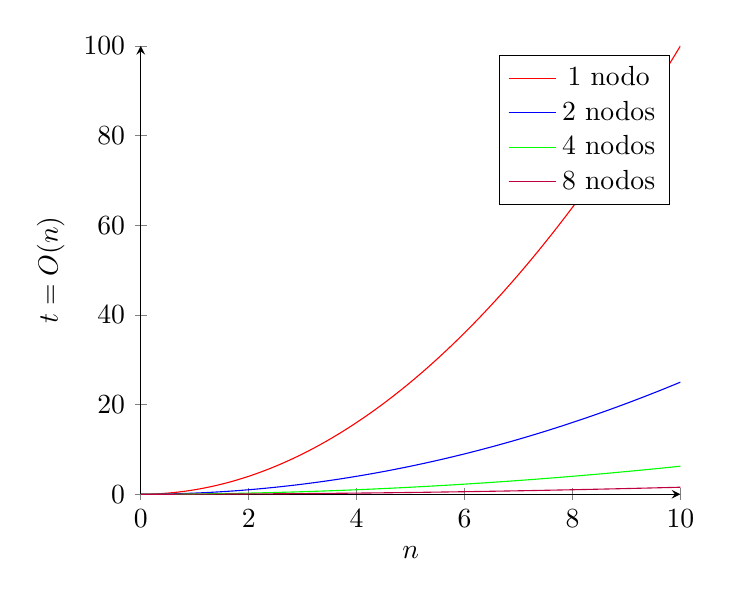
\begin{tikzpicture}
		\centering
		\begin{axis}[
			axis lines = left,
			xlabel = $n$,
			ylabel = {$t = O(n)$},
			]
			\addplot [domain=0:10, samples=100, color=red,] {x^2};
			\addlegendentry{1 nodo}

			\addplot [domain=0:10, samples=100, color=blue,]{x^2/4};
			\addlegendentry{2 nodos}

			\addplot [domain=0:10, samples=100, color=green,]{x^2/16};
			\addlegendentry{4 nodos}

			\addplot [domain=0:10, samples=100, color=purple,]{x^2/64};
			\addlegendentry{8 nodos}
		\end{axis}
	\end{tikzpicture}
	\caption{Aproximación de funciones de complejidad temporal según la cantidad de nodos del cluster de computadoras.}
	\label{fig:complejidad_temporal_figura}
\end{figure}

\bigskip La unidad básica de Apache Spark es llamada0 tarea, y la cantidad de tareas depende del número de particiones del conjunto de datos de entrada. Cada una de las tareas se encuentra en un hilo de ejecución de una JVM\footnote{Del inglés \textit{Java Virtual Machine}, es una máquina virtual que permite ejecutar programas en código intermedio Java.}, dedicado exclusivamente a un \textit{ejecutor}. Uno o más ejecutores son desplegados en los distintos \textit{nodos} del cluster de computadoras \citep{janardhanan2020optimum}. Es decir, que el paralelismo obtenido por la infraestructura Spark, depende de los tres niveles: tareas, ejecutores y nodos; así como también de la naturaleza del algoritmo que se ejecuta en la misma. Con el fin de dar un ejemplo aplicable al cálculo de similaridad, se configura un cluster de computadoras de 4 nodos, y 4 ejecutores en cada uno de ellos. Si cada uno de los ejecutores asigna 1-14 núcleos de CPU de forma dinámica, el número total de núcleos variará entre 4 y 56. Esto significa, que habrá de 4 a 56 tareas ejecutándose paralelamente en la infraestructura definida.

\subsection{Implementación en un sistema de recomendación de tiempo real}

Como punto de partida a esta sección, se aclara que este trabajo de tesis no cubre la implementación del RS propiamente dicho. No obstante, persigue como objetivo el desarrollo de un nuevo método para implementar la matriz de similaridad asociada al RS, a partir de un gran volumen de datos de entrada, en particular en CQA, y utilizando una arquitectura Big Data. Para tal fin, se propondrá un ejemplo de RS a tiempo real, que dará contexto al trabajo en cuestión. El ejemplo será desarrollado teniendo en cuenta 3 casos de uso diferentes: \begin{enumerate*} [label=(\roman*)] \item un proceso batch ejecutado periódicamente que actualizará la base de datos, caso de uso central de este trabajo y en el cual se sustenta toda la arquitectura propuesta, y que también puede pensarse como una parte integrante de la implementación propuesta en este apartado; \item el punto de vista del usuario que consulta una pregunta en el sitio; y \item el caso  (opcional) en que el usuario agrega una nueva pregunta al sitio.\end{enumerate*}

\subparagraph{El proceso completo del sistema de recomendación}
La propuesta ejemplo de un sistema de recomendación completo se puede analizar teniendo en cuenta 3 casos de uso, uno de los cuales es el planteado en esta Tesis.

\bigskip El primer caso de uso consiste en un proceso que se ejecuta fuera de línea. El mismo es el encargado de actualizar las relaciones de similaridad entre todas las preguntas existentes en el sitio, utilizando el método EQuAL para perseguir tal fin, y utilizando la arquitectura Big data planteada. Además, es el responsable de entrenar los modelos de recomendación con cierta frecuencia. Este es el caso analizado en esta Tesis. El segundo caso de uso consiste en la consulta de una pregunta en el sitio. Este caso se nutre del caso de uso anterior, y utiliza sus resultados para obtener una lista de preguntas similares a la consultada. Por otro lado, si bien el procesamiento batch tiene en cuenta todas las preguntas existentes, no posee la capacidad de recomendar preguntas similares a una pregunta recién agregada al sistema en tiempo real (hasta que el mismo sea ejecutado nuevamente). Por lo anterior, el tercer caso de uso, que es opcional, se trata de una actualización en la que un usuario agrega una nueva pregunta al sitio, y la resolución como implementación tecnológica para recomendar preguntas similares en tiempo real.

\bigskip Se dará una propuesta de implementación de un RS completo, para dar contexto y tener una idea de funcionamiento en conjunto del mismo. En el mismo, se incluye como parte componente el método propuesto en esta Tesis y su arquitectura subyacente.

\bigskip
\begin{figure}[h!]
	\centering
	\includegraphics[width=0.9\linewidth]{8_problema_investigacion/imagenes/implementacion_rs}
	\caption{Arquitectura de un sistema de recomendación a tiempo real utilizando el método EQuAL.}
	\label{fig:implementacionrs}
\end{figure}

\subsubsection{Arquitectura general}
La arquitectura del RS embebido en un sitio de CQA colaborativo, consiste básicamente de un microservicio dedicado a recomendación, un artefacto de software que realizará la función de recomendación a tiempo real de forma distribuida, una base de datos altamente escalable NoSQL, y un proceso batch que generará una actualización de la misma de forma periódica.

La Figura \ref{fig:implementacionrs} muestra cómo interactúa la totalidad de componentes relativos al RS, divididos fundamentalmente en procesamiento a tiempo real y batch; y además, muestra todas las interacciones posibles entre los componentes. En los siguientes apartados, se explicará cada uno de los 3 casos de uso más importantes e identificables dentro de este sistema.

\subsubsection{Procesamiento batch}
La Figura \ref{fig:implementacionrsbatch} muestra el procesamiento batch para actualización y carga inicial de la base de datos que contendrá la matriz de co-asociación en un formato adecuado para consulta. Este proceso se ejecutará periódicamente, teniendo como entrada al conjunto de datos Quora en una base de datos (la misma debe ser inicializada con el conjunto de datos utilizado en este trabajo de tesis en forma de archivos de texto). A continuación se detallaran cada uno de los casos.

\bigskip
\begin{figure}[h!]
	\centering
	\includegraphics[width=0.9\linewidth]{8_problema_investigacion/imagenes/implementacion_rs_batch}
	\caption{Arquitectura de un sistema de recomendación a tiempo real utilizando el método EQuAL.}
	\label{fig:implementacionrsbatch}
\end{figure}

Como punto de partida y en solo una oportunidad, se carga una base de datos con el conjunto de datos Quora original. Esta base de datos podría ser relacional, o de otro tipo, pero debería tener dos características principales: rápida inserción de registros y debe permitir obtener todos los registros de una tabla mediante una sola consulta. La inserción rápida es importante en el caso del agregado de una nueva pregunta en tiempo real. Por otro lado, la capacidad de seleccionar todos los registros de una tabla, tiene importancia para el proceso batch que utilizara el método EQuAL para la actualización periódica del RS.

\bigskip De forma periódica el proceso batch, en el cual se basa este trabajo, obtendrá todas las preguntas de la base de datos de preguntas individuales para crear la matriz de co-asociación. La periodicidad podrá variar dependiendo de la configuración y la arquitectura en la cual se ejecuta, mientras más rápido sea, más frecuente podría ser programado. Podría ejecutarse diariamente, en momentos de bajo tráfico en el sitio en cuestión. Por otro lado, este proceso será el encargado de entrenar, de forma ad-hoc, los modelos que así lo requieran, generar nuevos corpus que se nutrirán de nuevas palabras provenientes de preguntas nuevas agregadas por los usuarios una vez que el sistema esté en funcionamiento.

\bigskip
\begin{table}[h!]
	\footnotesize
	\caption{Matriz de co-asociación salida del proceso EQuAL.}
	\begin{tabularx}{\textwidth}{*{7}{>{\centering\arraybackslash}X}}
		\toprule
		\textbf{question\_id\_1} & \textbf{question\_id\_2} & \textbf{question\_1} & \textbf{question\_2} & \textbf{similarity} \\
		\midrule
		1 & 2 & question\_desc\_1 & question\_desc\_2 & 0.34 \\
		1 & 3 & question\_desc\_1 & question\_desc\_3 & 0.67 \\
		1 & 4 & question\_desc\_1 & question\_desc\_4 & 0.92 \\
		\bottomrule
	\end{tabularx}
	\label{tab:table-co-asociation}
\end{table}

Adicionalmente, un proceso ETL\footnote{Siglas para Extract, Transform and Load «extraer, transformar y cargar».}, que tendrá como origen la matriz de co-asociación, cargará la base de datos que guardará la información de similaridad entre preguntas y es consultada por el servicio de recomendación.  Las características que debe tener esta base de datos serán descritas en el apartado siguiente. El proceso ETL podrá ser lanzado mediante un evento que indique que la nueva matriz de co-asociación ha sido generada, o bien podría ser una extensión del proceso EQuAL. Un ejemplo de la entrada de este procesamiento puede ser el que se muestra en la Tabla \ref{tab:table-co-asociation}, el cual muestra la matriz de co-asociación: las columnas \(question\_id\_1\) y \(question\_id\_2\) corresponden a los identificadores de preguntas, las columnas \(question\_1\) y \(question\_2\) corresponden al contenido de cada una de las preguntas, y la columna \(similarity\) indica cual es la similaridad entre las dos preguntas de cada una de las filas. Por ejemplo, la primera fila indica una similaridad de \(0.34\) entre las pregunta 1 y 2. Luego del proceso ETL, los registros de la base de datos para el RS tendrán la estructura que se muestra en la Tabla \ref{tab:table-similar-questions}, que posee solo tres columnas, el ID de pregunta (\(question\_id\)), su descripción (\(question\)), y la preguntas similares con su similaridad, cada una de las preguntas similares está compuesta por un ID, la descripción y la similaridad con la pregunta correspondiente a la fila en cuestión (\(similar\_questions\)). Esto permitirá consultar la pregunta mediante su ID de manera muy eficiente y veloz. Por otro lado, la carga de la tabla también será muy eficiente, ya que la cantidad de registros se reduce a la cantidad de preguntas individuales, en lugar de la cantidad de registros de la matriz de co-asociación. La columna “similar\_questions” será en formato JSON, lo cual permite acceder a datos con una estructura definida, y serializar y deserializar los mismos de una forma estándar.

\bigskip Además, este proceso ETL podría ser utilizado para la actualización de índices o matrices en memoria utilizadas para un RS a tiempo real.

\begin{table}[h!]
	\centering
	\footnotesize
	\caption{Ejemplo de un registro de la base de datos de similaridad entre preguntas.}
	\begin{tabular}{|c|c|l|}
		\hline
		\textbf{question\_id} &
		\textbf{question} &
		\multicolumn{1}{c|}{\textbf{similar\_questions}} \\ \hline
		1 & question\_desc\_1 & \begin{lstlisting}[language=json]
[
	{
		"id": 4,
		"question": "question_desc_4",
		"similarity": "0.92"
	},
	{
		"id": 3,
		"question": "question_desc_3",
		"similarity": "0.67"
	},
	{
		"id": 2,
		"question": "question_desc_2",
		"similarity": "0.34"
	}
]
		\end{lstlisting} \\ \hline
	\end{tabular}
	\label{tab:table-similar-questions}
\end{table}

\subsubsection{Consulta de una pregunta existente}
En este apartado, se supone que la base de datos posee toda la información necesaria y está disponible; y además, que existe una aplicación web que consulta un servicio backend dedicado al sistema de recomendación, mediante una API REST\footnote{Representational State Transfer. Es una arquitectura y conjuntos de convenciones basada en servicios web para intercambios de información.}. Este último consultará la base de datos para devolver las preguntas similares a un ID de pregunta dado.

\begin{figure}[h!]
	\centering
	\includegraphics[width=0.6\linewidth]{8_problema_investigacion/imagenes/implementacion_rs_consulta}
	\caption{Flujo de consulta de una pregunta existente.}
	\label{fig:implementacionrsconsulta}
\end{figure}

La Figura \ref{fig:implementacionrsconsulta} muestra el flujo de la consulta de una pregunta existente. En el momento que un usuario consulta una pregunta en el sitio, el servicio frontend enviará una solicitud GET al servicio backend, utilizando el ID de la pregunta en cuestión. El servicio backend buscará la pregunta en la base de datos utilizando el ID de pregunta y retornando todas las preguntas similares. Las preguntas similares correspondientes, pueden estar ordenadas por el valor de similaridad en forma decreciente. Esta operación debería ser ejecutada de manera rápida y eficiente, debido a que el servicio backend es dedicado al RS y la base de datos posee las siguientes características:
\begin{enumerate}
	\item La información de similaridad entre preguntas estará almacenada en una tabla con una clave primaria simple (PK), formada solo por el ID de pregunta. Esta estructura genera un índice por ID de pregunta, lo cual posibilita una búsqueda rápida.
	\item La tabla anteriormente mencionada podría estar particionada por la PK. Esto significa que se generan particiones de datos a lo largo de los diferentes nodos en el esquema de base de datos, basado en una función hash consistente y generada por el ID de pregunta. Esto es especial para búsquedas rápidas por PK, y además, facilita la escalabilidad horizontal y replicación.
	\item La información de preguntas similares para un ID dado, estará en formato JSON, haciendo que el servicio backend tenga un trabajo casi nulo para disponibilizar las preguntas similares al usuario final.
	\item Se recomienda una base de datos NoSQL ya que ellas vienen con un número de buenas prácticas arquitectónicas que afectan el rendimiento, tales como, distribución de datos automáticas, baja latencia, consultas asíncronas, replicación de datos y alta disponibilidad.
\end{enumerate}

\subsubsection{Agregar una nueva pregunta}
Esta funcionalidad es opcional y depende de los requerimientos del sitio y las funciones de recomendación a desarrollar, ya que recomendar ítems instantáneamente a uno recién agregado a un RS es un gran desafío para los arquitectos de software. Cabe aclarar que esta funcionalidad es opcional ya que, si los requerimientos del sistema no requieren de la misma, se podría esperar que el proceso batch sea ejecutado, y asigne preguntas similares a la pregunta recién agregada. El propósito principal es el cálculo en tiempo real de los ítems recomendados para el ítem recién agregado al sistema, hacerlos disponibles al usuario final, y que esto no signifique una sobrecarga del mismo. La recomendación en tiempo real será provisoria hasta que esta pregunta sea tenida en cuenta por el proceso batch y se encuentre disponible en la base de datos del RS, por lo cual, esta funcionalidad puede ser utilizada como respaldo en el caso de que una pregunta no sea encontrada en dicha base de datos. La arquitectura propuesta a continuación, que se detalla en la Figura \ref{fig:implementacionrsagregar}, propone el cálculo de similaridad a tiempo real, utilizando métodos derivados del método EQuAL que sean apropiados y tengan buen desempeño. Esto permitirá que, no solo los usuarios del sitio puedan tener acceso a las mismas de manera inmediata, sino que también sean accesibles al mismo usuario que agregó la pregunta, evitando así, con suerte, el tiempo de espera en que su pregunta sea respondida.

\begin{figure}[h!]
	\centering
	\includegraphics[width=0.9\linewidth]{8_problema_investigacion/imagenes/implementacion_rs_agregar}
	\caption{Flujo en el RS a tiempo real cuando se agrega una nueva pregunta al sistema.}
	\label{fig:implementacionrsagregar}
\end{figure}

\bigskip Cuando se agrega una nueva pregunta, la información es enviada al servicio backend mediante una solicitud POST, el cual es enviado al módulo que realiza el cálculo de recomendación a tiempo real. Este último, retorna las preguntas similares para que estén disponibles al usuario. Luego de efectuar la pregunta, el usuario puede ser redireccionado a una URL que contenga la pregunta recién agregada y las preguntas similares. Por otro lado, y de manera asíncrona, el servicio backend guarda la pregunta recién agregada a la base de datos de preguntas individuales, para que sea tenida en cuenta en la próxima ejecución del proceso batch.

\bigskip El módulo de recomendación en tiempo real podría realizar el cálculo de recomendación con distintos enfoques. A continuación, se mencionan propuestas, que quedan fuera del alcance de esta tesis, para implementar arquitecturas de buen desempeño utilizando enfoque de Big Data.

\subparagraph{Cálculo de similaridad contra todas las preguntas del sitio}
En este enfoque, de ser posible, este módulo debería mantener la matriz de co-asociación en memoria, para poder realizar el cálculo a demanda. La pregunta recién ingresada debe compararse con todas las preguntas del sitio. Al mismo tiempo, se quiere tener control del tamaño de la matriz. Para tal fin, es posible mantener solo una fracción de la misma con los datos más importantes. Existen diversas técnicas para llevarlo a cabo, por ejemplo implementar un algoritmo de \textit{Caché de Reemplazo Adaptativo }(ARC\footnote{Por sus siglas en inglés \textit{Adaptive Replacement Cache}.}) que descarta los objetos que no fueron usados recientemente y los objetos con menor frecuencia de uso. Por otro lado, las preguntas, como se describió anteriormente, deben tener un ID único. Por lo cual, cada registro en el caché puede ser asignado a una pregunta. Con IDs en el rango \(0.. N-1\) si \(N\) es la cantidad total de registros en el caché.

\bigskip En cuanto al cálculo de similaridad, los modelos que lo requieran, deben estar pre-entrenados y cargados en memoria. Por ejemplo, podría ser posible que una nueva pregunta realice una comparación con todas las preguntas en caché (fuerza bruta) utilizando cada uno de los algoritmos de similaridad. El proceso de ensamble de clustering puede ser simplificado a la media de los valores calculados por los algoritmos de similaridad subyacentes, para luego retornar las k preguntas más similares a la recién agregada.

\subparagraph{Búsqueda de vecinos cercanos con representaciones vectoriales}
Este enfoque utiliza representaciones vectoriales de cada una de las preguntas individuales. Para tal fin, es posible que el método EQuAL que se ejecuta periódicamente genere una representación vectorial de cada una de las preguntas, utilizando uno de los métodos (o varios de ellos combinados) que usan este tipo de representación como paso intermedio del cálculo de similaridad. Con este listado de preguntas en forma de vector, es posible cargar un índice en memoria que permita la búsqueda de un conjunto de vectores inmediatamente.

\bigskip Mediante una nueva pregunta agregada al sistema y su representación vectorial, es posible buscar sus \(k\) vecinos más cercanos. Este método de clasificación es llamado \textit{KNN} (del inglés \textit{k-Nearest-Neighbors}). Para un registro \(t\) a ser clasificado, sus \(k\) vecinos más cercanos son obtenidos en la forma de vecinos de \(t\) \citep{guo2003knn}. Este método es utilizado por varias librerías reconocidas por la industria, tales como Annoy \footnote{Spotify Annoy GitHub Repository: \url{https://github.com/spotify/annoy}. Último acceso: Junio 2021.}, las cuales poseen un muy buen desempeño, realizan un uso muy eficiente de memoria.

\subparagraph{Modelos de scoring}
Es posible utilizar el proceso ETL parte del procesamiento batch para cargar un motor de búsqueda que contenga índices basados en scoring. Ciertas herramientas, tales como ElasticSearch\footnote{Sitio web ElasticSearch: \url{https://www.elastic.co/}. Último acceso: Junio 2021.}, tienen la capacidad de devolver documentos similares a uno consultados basándose en la generación de índices. El listado de preguntas puede ser tomado como entrada para la generación del mismo. Cada uno de los documentos es indexado. Los términos presentes en cada una de las preguntas (documentos) son descompuestos e indexados de forma invertida. Cada término es  indexado, y contendrá, por ejemplo, en qué posición dentro de cada documento se encuentra. En el momento de una nueva consulta, se devuelven todos los documentos que coinciden con la misma. Con el fin de dar relevancia a los mismos, cada uno de los documentos tiene asignado un score que es calculado con el método TF-IDF (tal como se explicó anteriormente), es decir, que un término que se encuentra varias veces en el documento consultado pero es contenido por pocos documentos en el índice, tendrá más relevancia que un término que aparece con más frecuencia en distintos documentos. Entonces, la relevancia de cada uno de los documentos retornados, depende (en parte) del peso de cada término en el documento consultado.

\subsubsection{Condiciones institucionales para el desarrollo de la tesis. Infraestructura y equipamiento}
El presente trabajo se lleva a cabo en el marco del Proyecto PID UTN: Minería de Datos aplicado a problemáticas de Big Data de la Universidad Tecnológica Nacional, Facultad Regional Rosario\footnote{Código del PID: SIUTNRO0005006. Bajo la dirección del Ing. Eduardo Amar.}.

\bigskip El candidato cursó la Maestría en Ingeniería en Sistemas de Información en dicha Facultad y tendrá a disposición el equipamiento e instalaciones del Departamento en Ingeniería en Sistemas de Información. Con el objetivo de realizar el desarrollo tecnológico de este trabajo de tesis, el candidato utilizará equipos propios así como también los equipos de la universidad, en caso de que sea necesario. Los conjuntos de datos para la experimentación y validación de la solución propuesta están disponibles libremente en Internet, así como también el software y herramientas necesarias.





















	\chapter*{Experimentos}\label{ch:experimentos}
\addcontentsline{toc}{chapter}{Capitulo 5. Experimentos}

\section*{Experimentos}
\addtocounter{section}{1}
\setcounter{subsection}{0}

\subsection{Estado del arte}
El proyecto en el cual se realizaron los experimentos que este trabajo tiene como estado del arte, es un proyecto basado en código Python que se puede encontrar en el siguiente repositorio GitHub \url{https://github.com/Departamento-Sistemas-UTNFRRO/text_comparison}.

\bigskip Tiene como características principales la utilización de los 5 algoritmos de similaridad mencionados anteriormente (y evaluados a continuación) y la ejecución de cada uno de ellos en el marco de un patrón master-worker en un solo microprocesador. Este patrón es utilizado para el procesamiento paralelo, en el cual una tarea es enviada a cada uno de los “workers” para ser procesada. En este caso en particular, la cantidad de “workers” es fija y especificada como un parámetro en tiempo de ejecución.

\subsubsection{Análisis de rendimiento}
Se muestra al análisis de rendimiento para el cálculo de distancias con los el proyecto del estado del arte, con el fin de tener un punto comparativo para los experimentos que se realizarán con la nueva arquitectura. Las pruebas de los algoritmos de similaridad de rendimiento se realizaron con el siguiente equipo:

\begin{verbatim}
Modelo: MacBook Pro
Procesador: Intel Core i7
Velocidad del procesador: 2.6 GHz
Numero de nucleos: 6
Caché L2 (por núcleo): 256 KB
Caché L3: 12 MB
Tecnología Hyper-Threading: Habilitada
Memoria: 16 GB RAM
Almacenamiento: APPLE SSD AP0512M
\end{verbatim}

El cual también será utilizado para las pruebas de la nueva arquitectura. Se utilizará, como parámetro de rendimiento, el cálculo de similaridad para cada uno de los 404290 pares de preguntas. Luego de varias pruebas, se llega a una configuración de 8 hilos de ejecución y lotes de 10000 pares de preguntas, para obtener los tiempos más bajos posibles con cada uno de los algoritmos, los mismos fueron:

\subparagraph{Bag of Words}
\begin{verbatim}
[13:34:51] Starting script.
[13:34:51] Loading Quora questions file...
[13:34:52] ----- Run number 1 ------
[13:34:56] First 100000 distances calculated.
[13:34:58] First 200000 distances calculated.
[13:35:01] First 300000 distances calculated.
[13:35:03] First 400000 distances calculated.
[13:35:04] First 404290 distances calculated.
[13:35:04] Script finished. Total time: 0:00:12.895492
\end{verbatim}

\subparagraph{TF/IDF}
\begin{verbatim}
[13:31:05] Starting script.
[13:31:05] Loading Quora questions file...
[13:31:07] ----- Run number 1 ------
[13:31:07] Generating a sample of 0 questions.
[13:31:08] Training model...
[13:32:43] First 100000 distances calculated.
[13:33:20] First 200000 distances calculated.
[13:33:58] First 300000 distances calculated.
[13:34:38] First 400000 distances calculated.
[13:34:39] First 404290 distances calculated.
[13:34:39] Script finished. Total time: 0:03:33.665420
\end{verbatim}

\subparagraph{FastText}
\begin{verbatim}
[13:39:25] Starting script.
[13:39:25] Loading Quora questions file...
[13:39:26] ----- Run number 1 ------
[13:39:28] Training model...
Read 9M words
Number of words:  30823
Number of labels: 0
Progress: 100.0% words/sec/thread:  147553 lr:  0.000000 loss:  1.791601 ETA:   0h 0m
[13:40:29] First 100000 distances calculated.
[13:40:47] First 200000 distances calculated.
[13:41:06] First 300000 distances calculated.
[13:41:24] First 400000 distances calculated.
[13:41:25] First 404290 distances calculated.
[13:41:25] Script finished. Total time: 0:02:00.335008
\end{verbatim}

\subparagraph{Word2Vec}
\begin{verbatim}
[13:42:29] Starting script.
[13:42:29] Loading Quora questions file...
[13:42:30] ----- Run number 1 ------
[13:42:34] First 100000 distances calculated.
[13:42:36] First 200000 distances calculated.
[13:42:38] First 300000 distances calculated.
[13:42:39] First 400000 distances calculated.
[13:42:40] First 404290 distances calculated.
[13:42:40] Script finished. Total time: 0:00:10.719605
\end{verbatim}

\subparagraph{Semantic Distance}
\begin{verbatim}
[16:04:34] Starting script.
[16:04:34] Loading Quora questions file...
[16:04:35] ----- Run number 1 ------
[16:26:11] First 100000 distances calculated.
[16:47:20] First 200000 distances calculated.
[17:08:41] First 300000 distances calculated.
[17:30:08] First 400000 distances calculated.
[17:31:06] First 404290 distances calculated.
[17:31:06] Script finished. Total time: 1:26:32.941992
\end{verbatim}

\begin{table}[h!]
		\footnotesize
		\caption{Análisis de rendimiento de los algoritmos de similaridad del estado del arte.}
		\begin{tabularx}{\textwidth}{*{7}{>{\centering\arraybackslash}X}}
		\toprule
		& \textbf{Tiempo total (segundos)} & \textbf{Velocidad aproximada (calc/seg)} \\
		\midrule
		\textbf{Bag of words} & 12.895492 & 31351.26601 \\
		\textbf{TF/IDF} & 213.66542 & 1892.163926 \\
		\textbf{FastText} & 120.335008  & 3359.703936 \\
		\textbf{Word2Vec}  & \textbf{10.719605} & \textbf{37715.00909} \\
		\textbf{Semantic Distance} & 5192.941992 & 77.85374853 \\
		\bottomrule
	\end{tabularx}
	\label{tab:performance-estado-del-arte}
\end{table}

Los resultados en Tabla \ref{tab:performance-estado-del-arte} muestran una clara ventaja en términos de rendimiento para el algoritmo de similaridad Word2Vec (con un tiempo total de \(10.719605\) segundos, marcado en negrita), inmediatamente seguido por Bag of Words. TF/IDF y FastText, muestran un rendimiento aceptable pero, en comparación, aproximadamente diez veces más lentos que los anteriormente mencionados. El rendimiento del algoritmo de similaridad Semantic Distance, es muy bajo y representa un gran problema al momento de analizar grandes conjuntos de datos, pero puede ser necesario utilizarlo debido a sus buenas medidas de desempeño y error y su análisis de similaridad desde una perspectiva distinta.

\subsubsection{Medidas de desempeño y error}
Utilizando cada para de preguntas del conjunto de datos original, se calculó la matriz de confusión para cada uno de los algoritmos de similaridad, a través del método de validación explicado en la sección \ref{estructurasconfusion}. Como se puede ver en la Tabla \ref{tab:desempeno-estado-del-arte}.

\begin{table}[h!]
	\footnotesize
	\caption{Matrices de confusión para los cinco algoritmos de medidas de similaridad.}
	\begin{tabularx}{\textwidth}{*{7}{>{\centering\arraybackslash}X}}
		\toprule
		\multicolumn{3}{l}{\multirow{2}{*}{}} &
		\multicolumn{2}{c}{\textbf{Predicho}} &
		\multirow{2}{*}{\textbf{Exactitud}} &
		\multirow{2}{*}{\textbf{Error}} \\ \cmidrule(lr){4-5}
		\multicolumn{3}{l}{} &
		\multicolumn{1}{c}{\textbf{0}} &
		\multicolumn{1}{c}{\textbf{1}} &
		&
		\\ \midrule
		\multicolumn{1}{c}{\multirow{2}{*}{\textbf{TF}}} &
		\multicolumn{1}{c}{\multirow{2}{*}{\textbf{Real}}} &
		\multicolumn{1}{c}{\textbf{0}} &
		\multicolumn{1}{c}{0.4355} &
		\multicolumn{1}{c}{0.1953} &
		\multicolumn{1}{c}{\multirow{2}{*}{0.6776}} &
		\multicolumn{1}{c}{\multirow{2}{*}{0.3224}} \\ \cmidrule(lr){3-5}
		\multicolumn{1}{c}{} &
		\multicolumn{1}{c}{} &
		\multicolumn{1}{c}{\textbf{1}} &
		\multicolumn{1}{c}{0.1271} &
		\multicolumn{1}{c}{0.2421} &
		\multicolumn{1}{c}{} &
		\multicolumn{1}{c}{} \\ \midrule
		\multicolumn{1}{c}{\multirow{2}{*}{\textbf{TF/IDF}}} &
		\multicolumn{1}{c}{\multirow{2}{*}{\textbf{Real}}} &
		\multicolumn{1}{c}{\textbf{0}} &
		\multicolumn{1}{c}{0.4477} &
		\multicolumn{1}{c}{0.1831} &
		\multicolumn{1}{c}{\multirow{2}{*}{0.6685}} &
		\multicolumn{1}{c}{\multirow{2}{*}{0.3315}} \\ \cmidrule(lr){3-5}
		\multicolumn{1}{c}{} &
		\multicolumn{1}{c}{} &
		\multicolumn{1}{c}{\textbf{1}} &
		\multicolumn{1}{c}{0.1484} &
		\multicolumn{1}{c}{0.2208} &
		\multicolumn{1}{c}{} &
		\multicolumn{1}{c}{} \\ \midrule
		\multicolumn{1}{c}{\multirow{2}{*}{\textbf{Word2Vec}}} &
		\multicolumn{1}{c}{\multirow{2}{*}{\textbf{Real}}} &
		\multicolumn{1}{c}{\textbf{0}} &
		\multicolumn{1}{c}{0.4343} &
		\multicolumn{1}{c}{0.1965} &
		\multicolumn{1}{c}{\multirow{2}{*}{0.6788}} &
		\multicolumn{1}{c}{\multirow{2}{*}{0.3212}} \\ \cmidrule(lr){3-5}
		\multicolumn{1}{c}{} &
		\multicolumn{1}{c}{} &
		\multicolumn{1}{c}{\textbf{1}} &
		\multicolumn{1}{c}{0.1247} &
		\multicolumn{1}{c}{0.2445} &
		\multicolumn{1}{c}{} &
		\multicolumn{1}{c}{} \\ \midrule
		\multicolumn{1}{c}{\multirow{2}{*}{\textbf{FastText}}} &
		\multicolumn{1}{c}{\multirow{2}{*}{\textbf{Real}}} &
		\multicolumn{1}{c}{\textbf{0}} &
		\multicolumn{1}{c}{0.5033} &
		\multicolumn{1}{c}{0.1275} &
		\multicolumn{1}{c}{\multirow{2}{*}{0.6725}} &
		\multicolumn{1}{c}{\multirow{2}{*}{0.3275}} \\ \cmidrule(lr){3-5}
		\multicolumn{1}{c}{} &
		\multicolumn{1}{c}{} &
		\multicolumn{1}{c}{\textbf{1}} &
		\multicolumn{1}{c}{0.2} &
		\multicolumn{1}{c}{0.1692} &
		\multicolumn{1}{c}{} &
		\multicolumn{1}{c}{} \\ \midrule
		\multicolumn{1}{c}{\multirow{2}{*}{\textbf{Semantic Distance}}} &
		\multicolumn{1}{c}{\multirow{2}{*}{\textbf{Real}}} &
		\multicolumn{1}{c}{\textbf{0}} &
		\multicolumn{1}{c}{0.4877} &
		\multicolumn{1}{c}{0.1431} &
		\multicolumn{1}{c}{\multirow{2}{*}{\textbf{0.6797}}} &
		\multicolumn{1}{c}{\multirow{2}{*}{\textbf{0.3203}}} \\ \cmidrule(lr){3-5}
		\multicolumn{1}{c}{} &
		\multicolumn{1}{c}{} &
		\multicolumn{1}{l}{1} &
		\multicolumn{1}{l}{0.1772} &
		\multicolumn{1}{l}{0.192} &
		\multicolumn{1}{c}{} &
		\multicolumn{1}{c}{} \\ \bottomrule
	\end{tabularx}
	\label{tab:desempeno-estado-del-arte}
\end{table}

\bigskip Los resultados porcentuales de las matrices de confusión se muestran en cada intersección de filas y columnas. Los resultados reales se muestran en las filas, siendo los dos posibles 0, cuando las preguntas son distintas y 1 cuando las preguntas son iguales. Los resultados predichos, se muestran en las columnas.
La exactitud obtenida de las matrices de confusión, que se calcula como la suma de los resultados acertados entre los valores predichos y reales, en todos los casos exceden el \(66\%\), alcanzando un máximo de \(68\% \) para Word2Vec. Por otro lado, con respecto al error promedio, se llega a un valor máximo de \(33\%\) en el caso de TF/IDF.

\bigskip Observando las matrices de confusión, se presenta un desbalance en los dos valores tomados para calcular la exactitud, siendo que los resultados obtenidos para la clase “0” considerablemente mejores que para la clase “1”. Por ejemplo, el desbalance más grande se encuentra en la matriz de confusión de FastText, el cual es \(0,504 – 0,170 = 0,334\). Este tipo de desbalance puede ser originado por la distribución del conjunto de datos de entrada (\(36,9\%\) pares de preguntas son clase 1 y el \(63,1\%\) restante es clase 0), el cual pretende ser corregido con un método de muestreo explicado más adelante.















\subsection{Preprocesamiento del conjunto de datos}
\subsection{Muestreo del conjunto de datos}

Se generan muestras del conjunto de datos original en forma de subconjuntos del mismo. Cada uno de los subconjuntos, es generado de forma pseudo-aleatoria utilizando la función sample del paquete random, de la librería Python. De tal forma, se generan listas de tamaño \(N\) de elementos únicos seleccionados del total de la población de pares de preguntas.

\bigskip Cada uno de los subconjuntos de muestreo tiene un criterio de aceptación, la proporción de pares de preguntas iguales (con indicador 1) debe ser parecida a la proporción de preguntas distintas (con indicador 0); por lo cual, un subconjunto de muestreo es aceptado cuando la proporción de preguntas iguales está entre el \(35\%\) y \(75\%\) del total de preguntas del subconjunto. Esto garantiza que cada uno de los subconjuntos sea estadísticamente significativo y posea una variabilidad de datos tal que derive en resultados confiables.

\subsection{Generación de particiones}
\subsubsection{Cálculo de similaridades}
Se generaron particiones desde los subconjuntos de muestreos generados desde el conjunto de datos original. Teniendo en cuenta que se utilizó un algoritmo de clustering para desarrollar el método de este trabajo, fue necesario descomponer la estructura de los archivos de entrada ---el cual contiene un identificador por cada par de preguntas--- en preguntas individuales, con el fin de poder identificarlas unívocamente y utilizarlas como los objetos de entrada del análisis de clustering. La estructura de los subconjuntos de muestreo se clarifica en la Tabla \ref{tab:archivo-entrada}. Cada una de las filas contiene un identificador secuencial \(sequence\_id\), el identificador de par de preguntas proveniente del conjunto de datos original \(question\_pair\_id\), y las dos preguntas correspondientes \(question\_1\) y \(question\_2\).

\begin{table}[h!]
	\footnotesize
	\caption{Ejemplo de la estructura de los subconjuntos de muestreo.}
	\begin{tabularx}{\textwidth}{*{7}{>{\centering\arraybackslash}X}}
		\toprule
		\textbf{question\_pair\_id} & \textbf{question\_1} & \textbf{question\_2} \\
		\midrule
		123004                      & question\_0         & question\_2         \\
		98776                       & question\_1         & question\_3         \\
		\bottomrule
	\end{tabularx}
	\label{tab:archivo-entrada}
\end{table}

Luego, el conjunto el subconjunto de preguntas preparado para el cálculo de distancia fue generado de la siguiente forma:
\begin{enumerate}
	\item Se crea una matriz con la unión de las columnas \(question\_1\) y \(question\_2\), generando una fila por cada pregunta individual y un número secuencial que las identifica, como se muestra en la Tabla \ref{tab:preguntas-individuales}.
	\item Se realiza una combinación de cada una de las filas contra la matriz en sí misma (eliminando resultados repetidos).
\end{enumerate}

\begin{table}[h!]
	\footnotesize
	\caption{Ejemplo de la estructura del conjunto de preguntas individuales de la muestra en curso.}
	\begin{tabularx}{\textwidth}{*{7}{>{\centering\arraybackslash}X}}
		\toprule
		\textbf{sequence\_id} & \textbf{question} \\
		\midrule
		0                     & question\_0       \\
		1                     & question\_1       \\
		2                     & question\_2       \\
		3                     & question\_3       \\
		\bottomrule
	\end{tabularx}
	\label{tab:preguntas-individuales}
\end{table}

\begin{table}[h!]
	\footnotesize
	\caption{Combinación  de todas las preguntas individuales de una muestra.}
	\begin{tabularx}{\textwidth}{*{7}{>{\centering\arraybackslash}X}}
		\toprule
		\textbf{sequence\_id\_1} & \textbf{question\_id\_1} & \textbf{sequence\_id\_2} & \textbf{question\_id\_2} \\
		\midrule
		0 & question\_0 & 1 & question\_1 \\
		0 & question\_0 & 2 & question\_2 \\
		0 & question\_0 & 3 & question\_3 \\
		1 & question\_1 & 2 & question\_2 \\
		1 & question\_1 & 3 & question\_3 \\
		2 & question\_2 & 3 & question\_3 \\
		\bottomrule
	\end{tabularx}
	\label{tab:matriz-triangular}
\end{table}

\bigskip La Tabla \ref{tab:matriz-triangular} da un ejemplo de la combinación de todas las preguntas individuales de la muestra, utilizando el identificador de secuencia y el contenido de cada una de ellas. Esta estructura sirve de entrada para el cálculo de similaridad para cada una de las técnicas previamente mencionadas. Consecuentemente, es posible realizar un cálculo de similaridad entre las dos preguntas que pertenecen a una misma fila, y agregar esta información a la estructura de datos anterior. La Tabla \ref{tab:matriz-similaridad} posee la misma estructura que la Tabla \ref{tab:matriz-triangular}, con el agregado del valor de similaridad entre el par de preguntas de cada una de las filas, en la columna \(similarity\).

\bigskip
\begin{table}[h!]
	\footnotesize
	\caption{Ejemplo de la estructura de matriz de similaridad en formato de tabla.}
	\begin{tabularx}{\textwidth}{*{7}{>{\centering\arraybackslash}X}}
		\toprule
		\textbf{sequence\_id\_1} & \textbf{question\_id\_1} & \textbf{sequence\_id\_2} & \textbf{question\_id\_2} & \textbf{similarity} \\
		\midrule
		0 & question\_0 & 1 & question\_1 & similarity\_01 \\
		0 & question\_0 & 2 & question\_2 & similarity\_02 \\
		0 & question\_0 & 3 & question\_3 & similarity\_03 \\
		1 & question\_1 & 2 & question\_2 & similarity\_12 \\
		1 & question\_1 & 3 & question\_3 & similarity\_13 \\
		2 & question\_2 & 3 & question\_3 & similarity\_23 \\
		\bottomrule
	\end{tabularx}
	\label{tab:matriz-similaridad}
\end{table}

Si se piensa el subconjunto de datos de la Tabla \ref{tab:matriz-similaridad} en forma de matriz, en lugar de estructura de tabla, al calcular la distancia de cada una de las filas, se estaría formando una \textit{matriz triangular superior}, en la cual cada uno de los elementos es la distancia entre un par de preguntas:
\[\begin{bmatrix}0 & similarity\_01 & similarity\_02 & similarity\_03 \\ 0 & 0 & similarity\_12 & similarity\_13  \\ 0 & 0  & 0 & similarity\_23  \\ 0 & 0 & 0 & 0 \end{bmatrix}.\]
La estructura de tabla, en lugar de una estructura matricial como la anterior, es utilizada por cuestiones de tecnología. Al utilizarse Python, Apache Spark y el sistema de archivos, es posible generar archivos delimitados por comas (archivos CSV) utilizando el soporte nativo que poseen las tecnologías anteriormente mencionadas. Adicionalmente, esto posibilitó crear particiones de datos de manera sencilla y procesarlas de forma distribuida.

\subsubsection{Clustering y etiquetado}
Una vez que las similaridades son calculadas en forma distribuida los resultados se almacenan y son colectados para realizar un etiquetado a partir de un análisis de clustering.

\bigskip El algoritmo elegido fue Clustering de Partición Alrededor de Medoides (PAM) como forma de “etiquetar” cada una de las preguntas como pertenecientes a un determinado cluster, por cada una de las ejecuciones. El motivo de esta elección es porque los elementos no pueden representarse de forma directa en un espacio dimensional, dado que se comparan elementos de texto. Por esta razón, se usa un método que pueda recibir una matriz de similaridad como entrada, y los medoides son elementos reales que se encuentran en el conjunto de datos original. Se implementó de la forma que se describe a continuación.

\paragraph{Entrada y configuración inicial}
Como entrada fue utilizada la matriz de similaridad resultado del paso anterior, que sirve para obtener las distancias precalculadas entre cada uno de los elementos que participan en el proceso de clustering. Además, en otro arreglo en memoria, se utilizó el conjunto de preguntas individuales con un identificador secuencial, con el fin de facilitar el algoritmo, tal como se muestra en la Tabla \ref{tab:preguntas-individuales}.

\bigskip Por cada una de las corridas de clustering (parámetro de configuración) se proporciona un \(k\) inicial, que representa al número de clusters (o medoides) que define el algoritmo, y en los cuales las preguntas son distribuidas (proceso de etiquetado); y además, son identificadas con un identificador único universal (UUID\footnote{Identificador único universal \url{https://es.wikipedia.org/wiki/Identificador\_\%C3\%BAnico_universal}} por sus siglas en inglés) con el fin de poder recuperar cada uno de los resultados cuando se realice el ensamble de Clustering de cada una de estas ejecuciones.

\paragraph{Proceso de clustering}
Como se mencionó anteriormente, el algoritmo PAM tiene dos etapas, denominadas BUILD y SWAP. El algoritmo realiza una cantidad de iteraciones máxima (parámetro configurable), y por cada una de ellas se realiza el proceso descrito a continuación.

\subparagraph{Generación de etiquetas (BUILD)}
La generación de etiquetas significa asignar un medoide a una pregunta en particular, con el objetivo del armado de clusters. Como cada medoide es exclusivamente representativo de un cluster, la asignación de un medoide a una pregunta es equivalente a la asignación de la pregunta al cluster correspondiente.
\begin{enumerate}
	\item Se obtiene su similaridad con cada uno de los medoides. Para esto, se busca cada par de preguntas en una de las matrices de similaridad generadas por el paso anterior.
	\item Se asigna la pregunta al medoide (cluster) en la cual su similaridad es máxima.
	\item Se obtiene la suma de las similaridades totales por cada medoide, y se almacena en un arreglo que será utilizado en el siguiente paso.
	\item Se generan pares (ID pregunta, ID pregunta medoide) que representarán las etiquetas utilizadas por el algoritmo de ensamble.
\end{enumerate}

\subparagraph{Actualización de medoides (SWAP)}
Se busca actualizar los medoides con el fin de evaluar si, luego del cambio, se consiguen mejores resultados. Esto es, por cada uno de los clusters, se obtiene la similaridad de las preguntas todas contra todas, de la siguiente manera:

\begin{enumerate}
	\item Se toma una pregunta \(i\) de la lista, y se compara la similaridad con todas las preguntas restantes del cluster.
	\item Se suman todas las similaridades calculadas.
	\item Si esta suma es mayor a la suma de las similaridades que obtuvo el medoide actual en el paso anterior, la pregunta \(i\) pasa a ser el nuevo medoide.
	\item Se recalculan las etiquetas \((id\_pregunta, id\_pregunta\_medoide)\)
\end{enumerate}

La \textit{generación de etiquetas} y la \textit{actualización de medoides} se realizan de forma iterativa hasta que \begin{enumerate*} [label=(\roman*)] \item los medoides convergen o; \item se llega al límite máximo de iteraciones.\end{enumerate*} La convergencia de medoides significa que los medoides calculados por la iteración actual, son exactamente los mismos que la iteración anterior, lo que indica que el resultado es óptimo (dentro de los parámetros y las capacidades del algoritmo). Por otro lado, en caso de que no se haya conseguido la convergencia, el conjunto de clusters generado en la última iteración es el que se toma como válido.

\paragraph{Estructura de los resultados}
Los resultados son almacenados en un archivo CSV que posee la estructura de la Tabla \ref{tab:salida-clustering}. La primera columna es un UUID que identifica una ejecución en particular del algoritmo de clustering, la segunda columna es un identificador de pregunta individual, y la tercera columna es un identificador de pregunta real que actúa como medoide de un cluster.

\begin{table}[h!]
	\footnotesize
	\caption{Ejemplo de la estructura del resultado de la ejecución del algoritmo de clustering.}
	\begin{tabularx}{\textwidth}{ccc}
		\toprule
		\textbf{run\_uuid}                       & \textbf{question\_id} & \textbf{assigned\_medoid} \\
		\midrule
		63815467136575428551131593057064980770 & 336 & 856 \\
		63815467136575428551131593057064980770 & 342& 856 \\
		63815467136575428551131593057064980770 & 26 & 358 \\
		63815467136575428551131593057064980770 & 1364 & 437 \\
		\bottomrule
	\end{tabularx}
	\label{tab:salida-clustering}
\end{table}
Cada uno de los archivos almacena un UUID único (\(run\_uuid\)), es cual es idéntico en cada una de las filas, para facilitar el algoritmo de ensamble. Además, cada archivo contiene todas las preguntas individuales de la muestra en cuestión (\(question\_id\)), y el cluster a la cual pertenecen, el cual es representado por el ID de la pregunta que fue tomada como medoide para ese cluster (\(assigned\_medoid\)). Se generan tantos archivos por la cantidad de ejecuciones configuradas para cada una de las técnicas de similaridad del estado del arte. Por ejemplo, si utilizamos Word2Vec, TF, TFIDF, FastText y Semántica (5 técnicas) y se configuraron 100 ejecuciones por cada una de ellas, se obtendrán 500 archivos de etiquetas; los cuales serán la única entrada del algoritmo de ensamble de clustering.






\subsection{Ensamble de Clustering}
El proceso de ensamble comienza obteniendo todos los archivos de etiquetas generados por el paso anterior. El resultado es una estructura Spark, con la misma estructura que los archivos físicos, pero en memoria y en todos los nodos del cluster Hadoop, con el fin de poder realizar el procesamiento de una forma eficiente y escalable.

\bigskip El conjunto de etiquetas es agrupado por ID de pregunta, y se aplica una función de grupo que obtendrá una lista de tuplas o parejas  \((run\_id, cluster\_id)\). Con el fin de clarificar esta idea, se va a dar un ejemplo: Si se realizan 3 ejecuciones del algoritmo de clustering, cada una de ellas son representadas como archivos con formato CSV y procesada de manera distribuida. Cada uno de esos archivos generados para cada ejecución, contiene información del ID de ejecución y la asignación de cada una de las preguntas individuales a un cluster resultado. En el caso de PAM, cada identificador de cluster es un identificador real de una pregunta individual (o medoide desde la perspectiva algorítmica). En caso de que se realicen 3 ejecuciones, a modo de ejemplo, los archivos de etiqueta generados pueden representarse como se muestra en las Tablas \ref{tab:run1}, \ref{tab:run2} y \ref{tab:run3}, con identificadores de ejecución \(run\_uuid\_1\), \(run\_uuid\_2\) y \(run\_uuid\_3\), respectivamente.

\begin{table}[h!]
	\footnotesize
	\caption{Ejemplo de asignación de clusters a preguntas individuales para la ejecución 1.}
	\begin{tabularx}{\textwidth}{*{7}{>{\centering\arraybackslash}X}}
		\toprule
		\textbf{run\_uuid} & \textbf{question\_id} & \textbf{cluster\_id} \\
		\midrule
		run\_uuid\_1       & 1                     & 1                    \\
		run\_uuid\_1       & 2                     & 1                    \\
		run\_uuid\_1       & 3                     & 1                    \\
		run\_uuid\_1       & 4                     & 4                    \\
		\bottomrule
	\end{tabularx}
	\label{tab:run1}
\end{table}

\begin{table}[h!]
	\footnotesize
	\caption{Ejemplo de asignación de clusters a preguntas individuales para la ejecución 2.}
	\begin{tabularx}{\textwidth}{*{7}{>{\centering\arraybackslash}X}}
		\toprule
		\textbf{run\_uuid} & \textbf{question\_id} & \textbf{cluster\_id} \\
		\midrule
		run\_uuid\_2       & 1                     & 1                    \\
		run\_uuid\_2       & 2                     & 2                    \\
		run\_uuid\_2       & 3                     & 1                    \\
		run\_uuid\_2       & 4                     & 2                    \\
		\bottomrule
	\end{tabularx}
	\label{tab:run2}
\end{table}

\begin{table}[h!]
	\footnotesize
	\caption{Ejemplo de asignación de clusters a preguntas individuales para la ejecución 3.}
	\begin{tabularx}{\textwidth}{*{7}{>{\centering\arraybackslash}X}}
		\toprule
		\textbf{run\_uuid} & \textbf{question\_id} & \textbf{cluster\_id} \\
		\midrule
		run\_uuid\_3       & 1                     & 3                    \\
		run\_uuid\_3       & 2                     & 2                    \\
		run\_uuid\_3       & 3                     & 3                    \\
		run\_uuid\_3       & 4                     & 2                    \\
		\bottomrule
	\end{tabularx}
	\label{tab:run3}
\end{table}

Considerando \(run\_uuid\_1\), se puede observar que las preguntas 1, 2 y 3 fueron asignadas al cluster representado por la pregunta 1. En cambio, la pregunta 4 fue asignada a un cluster distinto, representado por la pregunta 3. La intuición para esta ejecución en particular, es que las preguntas 1, 2 y 3 son “más similares” entre sí, que la pregunta 4.

\bigskip En el siguiente paso, el conjunto de datos es agrupado por \(question\_id\), y se aplica una función de grupo que genera tuplas \((run\_id, cluster\_id)\). Para el ejemplo anterior resultaría tal como se muestra en la Tabla \ref{tab:tuplas}. La columna \(tuples\), contiene un arreglo de tuplas que indica, por cada pregunta individual, el conjunto de ocurrencias ejecución-cluster que fueron generadas a lo largo del experimento.

\begin{table}[h!]
	\footnotesize
	\caption{Conjunto de datos de asignación de clusters agrupados por pregunta individual para generación de tuplas \((run\_id, cluster\_id)\) .}
	\begin{tabularx}{\textwidth}{>{\centering\arraybackslash}p{2.0cm}>{\centering\arraybackslash}p{15cm}}
		\toprule
		\textbf{question\_id} & \textbf{tuples}                                          \\
		\midrule
		1                     & {[}(run\_uuid\_1,1),(run\_uuid\_2,1),(run\_uuid\_3,3){]} \\
		2                     & {[}(run\_uuid\_1,1),(run\_uuid\_2,2),(run\_uuid\_3,2){]} \\
		3                     & {[}(run\_uuid\_1,1),(run\_uuid\_2,1),(run\_uuid\_3,3){]} \\
		4                     & {[}(run\_uuid\_1,4),(run\_uuid\_2,2),(run\_uuid\_3,2){]} \\
		\bottomrule
	\end{tabularx}
	\label{tab:tuplas}
\end{table}

Hasta ahora, el conjunto de datos representado por la Tabla \ref{tab:tuplas} muestra, por cada una de las preguntas, a qué cluster fue asignada, por cada ejecución del algoritmo. Siguiendo con el ejemplo, la pregunta 1 y la pregunta 2 fueron asignadas al cluster con identificador 1 para \(run\_uuid\_1\) - ya que las dos preguntas poseen la tupla \((run\_uuid\_1,1)\) -. Este formato de representación, facilita el cálculo de la cantidad de veces que dos preguntas fueron asignadas al mismo cluster, para una misma ejecución. Para obtener el resultado de este cálculo, es necesario realizar una intersección de arreglos para cada una de las combinaciones de preguntas. Para este ejemplo, la intersección de arreglos se muestra en la Tabla \ref{tab:interseccion}.

\begin{table}[h!]
	\footnotesize
	\caption{Conjunto de datos intermedio que indica cuando dos preguntas coinciden en el mismo cluster/ejecución mediante un arreglo de tuplas.}
	\begin{tabularx}{\textwidth}{>{\centering\arraybackslash}p{2.5cm}>{\centering\arraybackslash}p{2.5cm}>{\centering\arraybackslash}p{10cm}}
		\toprule
		\textbf{question\_id\_1} & \textbf{question\_id\_2} & \multicolumn{1}{c|}{\textbf{tuples}}                     \\
		\midrule
		1 & 2 & {[}(run\_uuid\_1,1){]} \\
		1                        & 3                        & {[}(run\_uuid\_1,1),(run\_uuid\_2,1),(run\_uuid\_3,3){]} \\
		1 & 4 & {[}{]}                 \\
		2 & 3 & {[}(run\_uuid\_1,1){]} \\
		2 & 4 & {[}(run\_uuid\_2,2){]} \\
		3 & 4 & {[}{]}                 \\
		\bottomrule
	\end{tabularx}
	\label{tab:interseccion}
\end{table}

La longitud de cada una de las listas indica la cantidad de veces que una pregunta coincide con otra pregunta en el mismo cluster para una misma ejecución. Por ejemplo, las preguntas 1 y 3 resultaron en el mismo cluster para todas las ejecuciones, lo que indicaría una gran similaridad entre ellas. Por el contrario, las preguntas 1 y 4 no presentan ninguna intersección, lo cual es interpretado como una similaridad muy baja entre las preguntas en cuestión.

\bigskip La cantidad de veces que una pregunta coincide con otra, dividido la cantidad total de ejecuciones, nos indica, en un rango normalizado \([0,1]\), cuán similares son entre cada una de ellas, de manera adimensional. Aplicando esta teoría, calculamos:

\begin{python}
len(set(tuples_1).intersection(set(tuples_2))) / total_runs
\end{python}

Siendo el numerador de la expresión, la cantidad de veces que dos preguntas coincidieron en el mismo cluster para una misma ejecución, y el denominador la cantidad total de ejecuciones, respondiendo a la fórmula:
\[C(i,j)=\frac{n_{ij}}{N}\]

\bigskip Considerando el ejemplo en cuestión, el conjunto de datos resultado de aplicar la fórmula anterior se muestra en la Tabla \ref{tab:coasociacion}, que muestra la matriz de co-asociación de salida del proceso de ensamble de clustering. Esta matriz se compone de tres columnas, las dos primeras identifican a las preguntas y la tercera es la información de similaridad entre ellas.

\begin{table}[h!]
	\footnotesize
	\caption{Ejemplo de matriz de co-asociación salida del proceso de ensamble de clustering.}
	\begin{tabularx}{\textwidth}{*{7}{>{\centering\arraybackslash}X}}
		\toprule
		\textbf{question\_id\_1} & \textbf{question\_id\_2} & \textbf{similarity} \\
		\midrule
		1                        & 2                        & 0.3333              \\
		1                        & 3                        & 1.0                 \\
		1                        & 4                        & 0                   \\
		2                        & 3                        & 0.3333              \\
		2                        & 4                        & 0.3333              \\
		3                        & 4                        & 0                   \\
		\bottomrule
	\end{tabularx}
	\label{tab:coasociacion}
\end{table}
Particularmente, la matriz de co-asociación mostrada en la Tabla \ref{tab:coasociacion}, indica que las preguntas 1 y 3 coincidieron en el \(100\%\) de las ejecuciones, mientras que las preguntas 1 y 2 solo en un tercio de las mismas, y las preguntas 1 y 4 nunca coincidieron.

\subsection{Método de validación}\label{metodo-validacion}

\subsubsection{Generación de conjuntos estadísticamente significativos}

Para generar resultados estadísticamente significativos se ejecutó el proceso completo de modo iterativo, variando dos parámetros principales: \begin{enumerate*} [label=(\roman*)] \item el tamaño de la muestra y \item el número de clusters \(k\)\end{enumerate*}. Como experimentos para este trabajo se realizaron ejecuciones con conjuntos de datos aleatorios de 100, 500, 1000, 1500 y 2000 pares de preguntas (200, 1000, 2000, 3000 y 4000 preguntas individuales). Para cada tamaño de muestra, se realizaron 10 muestras aleatorias manteniendo un \(k\) fijo. Por ejemplo, para un número de clusters \(k = 5\) y para un tamaño de muestra 100, se realizaron 10 ejecuciones con un conjunto de datos de entrada aleatorio. Dando un total de \(5 \times 10 = 50\) matrices de co-asociación resultado, para un valor de \(k\) dado.

\paragraph{Elección de los tamaños de muestra}
En cuanto a la elección del tamaño de muestra en el apartado anterior, se tomó en cuenta que los conjuntos de datos sean lo suficientemente grandes como para generar resultados estadísticamente significativos, pero con un tamaño apropiado para la ejecución de los experimentos de forma local, en favor de la facilidad que para la depuración de los mismos. Cuando se aumenta el tamaño de la muestra en forma lineal, la cantidad de cómputos por cada uno de los algoritmos de similaridad aumentan de forma cuadrática. Como se mencionó anteriormente, Siendo \(n\) el número de pares de preguntas de una muestra, se realizarán \(2n^2-n\) cálculos. Además, si, por ejemplo, utilizamos 5 algoritmos de similaridad el número de cálculos de similaridad es de \(5(2n^2-n)\), con el agregado de que al algoritmos de clustering PAM y el ensamble de clustering también aumentan su complejidad de una forma considerable, dependiendo de nuestro número de clusters \(k\).

\paragraph{Elección del número de clusters}
La elección del número de clusters \(k\) en los experimentos realizados sigue una lógica que busca estandarizar a los mismos a lo largo de todos los tamaños de muestras, es decir, no variar el número de clusters entre ellas, con fines de comparación. Como regla general (\textit{rule of thumb} o \textit{regla del pulgar}) se considera como número ``óptimo'' de clusters un valor de alrededor de \(\sqrt{n/2}\) \citep{kodinariya2013review}, siendo \(n\) el tamaño de la muestra. Para el número de muestras elegido (200, 1000, 2000, 3000 y 4000 preguntas individuales), los valores siguiendo esta regla serían \(k = 10\), \(k = 22\), \(k = 31\), \(k = 38\), \(k =44\).

\bigskip Los valores generados por la regla del pulgar se encuentran en un rango \([10, 44]\), por lo cual, finalmente se optó por elegir los valores de \(k\) con una separación uniforme de los mismos, para facilitar su interpretación y visualización, respetando ese rango de cobertura. Los experimentos para este trabajo se realizaron con los valores \(k = 5, 10, 15, 20, 25, 30, 35, 40, 45, 50\).

\bigskip La validación de los valores de \(k\) elegidos para realizar los experimentos fueron validados en conjunto mediante el rendimiento de la matriz de co-asociación. Partiendo de la base del \textit{método del codo} para la evaluación del rendimiento de un algoritmo de clustering, el cual evalúa el porcentaje de variabilidad (suma de cuadrados de distancias) explicada en función del número de clusters, mediante la idea de encontrar el número mínimo de clusters por el cual agregando un cluster adicional no modelaría mejor los datos. El porcentaje de variabilidad explicado por los clusters es graficado contra el número de clusters. Los primeros clusters agregaran una información considerable al modelo, pero en cierto punto la ganancia marginal caerá dramáticamente, dando un ángulo en el gráfico \citep{bholowalia2014ebk}. La Figura \ref{fig:codo} muestra un gráfico bidimensional en el cual se compara el número de clusters (en abscisas) y la suma de cuadrados de distancias (en ordenadas) como medida de variabilidad de los clusters. En este gráfico se puede ver como luego de \(k = 5\), la suma de cuadrados de distancias varía muy poco, ya que los valores esbozan una curva con valores aproximadamente constantes a partir de este punto.

\begin{filecontents*}{codo.csv}
1,400
2,200
3,130
4,80
5,40
6,25
7,24
8,23
9,22
10,21
11,20
12,19
\end{filecontents*}

\begin{figure}
	\centering
	\scriptsize
	\resizebox{\textwidth}{!}{%
		\begin{tikzpicture}
			\begin{axis}[
				xlabel={Número de clusters (k)},
				ylabel={Suma de cuadrados de distancias},
				xmin=0, xmax=12,
				ymin=0, ymax=420,
				xtick={1,2,...,12},
				ytick={0,50,...,400},
				legend pos=north west,
				ymajorgrids=true,
				grid style=dashed,
				]

				\addplot table [mark=square,x index=0, y index=1, col sep=comma] {codo.csv};
				\label{codo}

				\draw [dashed] (50,0) -- (50,400);
			\end{axis}
		\end{tikzpicture}
	}
	\caption{Ejemplo de gráfico para método del codo. Valor óptimo \(k = 5\).}
	\label{fig:codo}
\end{figure}

\bigskip Con el fin de dar una aplicación más integral al método del codo, en lugar de calcularlo por cada una de las técnicas de clustering aplicadas, el mismo se aplicó utilizando la matriz de co-asociación generada a partir del ensamble. Para cuantificar y evaluar el rendimiento, se utilizó matrices de confusión que indican el error entre los resultados obtenidos y la clasificación proveniente del conjunto de datos original, por cada uno de los valores de \(k\) anteriormente mencionados.

\subsubsection{Estructura de las matrices de confusión}\label{estructurasconfusion}
Una matriz de confusión, es una matriz que muestra clasificaciones predichas y reales. Una matriz de confusión puede ser de tamaño \(L \times L\) donde \(L\) es el número de diferentes valores de etiqueta o clase \citep{provost1998glossary}. En este trabajo, las clases son: 0 (las preguntas comparadas no son iguales) y 1 (las preguntas son iguales). Por lo cual, la matriz de confusión que se deriva, se muestra en la Tabla \ref{tab:matriz-confusion}. Los valores “a” y “d” representan el porcentaje de veces que los valores predichos fueron iguales a los reales, es decir, los casos en que las preguntas fueron predichas, respectivamente, iguales o distintas y realmente lo eran. Por otro lado, “c” es la proporción de preguntas predichas distintas, que en realidad son iguales; y “b” la proporción de preguntas predichas iguales, pero son realmente distintas. El objetivo de un algoritmo con buen desempeño entonces, es maximizar “a” y “d” y, por lo tanto, minimizar “b” y “c”.

\bigskip
\begin{table}[h!]
	\footnotesize
	\centering
	\caption{Matriz de confusión para validación de resultados.}
	\begin{tabularx}{0.35\textwidth}{*{7}{>{\centering\arraybackslash}X}}
		\toprule
		\multicolumn{2}{l}{\multirow{2}{*}{}} & \multicolumn{2}{c}{\textbf{Predicho}}                             \\ \cmidrule(l){3-4}
		\multicolumn{2}{l}{}                  & \multicolumn{1}{c}{\textbf{0}} & \multicolumn{1}{c}{\textbf{1}} \\ \midrule
		\multicolumn{1}{c}{\multirow{2}{*}{\textbf{Real}}} & \multicolumn{1}{c}{\textbf{0}} & \multicolumn{1}{c}{a} & \multicolumn{1}{c}{b} \\ \cmidrule(l){2-4}
		\multicolumn{1}{c}{}  & \textbf{1}  & c                               & d                               \\ \bottomrule
	\end{tabularx}
	\label{tab:matriz-confusion}
\end{table}

Los indicadores de desempeño que se evaluaron en los experimentos realizados con fines comparativos, son los siguientes:
\begin{itemize}
	\item \textbf{Exactitud:} \((a+d)/(a+b+c+d)\)
	\item \textbf{Error:} \((b+c)/(a+b+c+d)\)
\end{itemize}
donde \(a+b+c+d=1\).

\paragraph{Preparación de los datos}
Para evaluar el rendimiento del algoritmo de ensamble, se toma la matriz de co-asociación generada como resultado del proceso total y la muestra de pares de preguntas que se utilizó como entrada para ese proceso. Por ejemplo, se considera la muestra de preguntas de la Tabla \ref{tab:muestra-validacion}, la cual muestra dos pares de preguntas (\(123004\) y \(98776\) - 4 preguntas en total) con su identificador de par y un indicador en la columna \(equal\), que tiene dos valores posibles: 1 (preguntas iguales) y 0 (preguntas distintas). Por otro lado, en la Tabla \ref{tab:coasociacion-validacion}, se muestra la matriz de co-asociación generada, por el método EQuAL, a partir de la Tabla \ref{tab:muestra-validacion}, teniendo en cuenta todas las combinaciones tomadas de a 2 de las 4 preguntas originales, para las cuales se agrega la similaridad entre pares, en la columna similarity. Por último, se filtran solo los pares de preguntas de la matriz de co-asociación que se encuentran en la Tabla \ref{tab:muestra-validacion}, ya que son las únicas con la cual su similaridad puede compararse con fines de validación, es decir, el conjunto de datos mostrado en la Tabla \ref{tab:filtrado-validacion}. Lo que nos deja con un conjunto de pares de preguntas que es posible comparar en su totalidad con la muestra original.

\begin{table}[h!]
	\footnotesize
	\centering
	\caption{Muestras de pares de preguntas que se utilizó como entrada del método EQuAL.}
	\begin{tabularx}{0.8\textwidth}{*{7}{>{\centering\arraybackslash}c}}
		\toprule
		\textbf{sequence\_id} & \textbf{question\_pair\_id} & \textbf{question\_1} & \textbf{question\_2} & \textbf{equal} \\
		\midrule
		0                     & 123004                      & question\_10         & question\_20         & 1              \\
		1                     & 98776                       & question\_11         & question\_21         & 0              \\
		\bottomrule
	\end{tabularx}
	\label{tab:muestra-validacion}
\end{table}

\begin{table}[h!]
	\footnotesize
	\caption{Matriz de co-asociación generada a partir de la muestra de la Tabla \ref{tab:muestra-validacion}.}
	\begin{tabularx}{\textwidth}{*{7}{>{\centering\arraybackslash}X}}
		\toprule
		\textbf{question\_id\_1} & \textbf{question\_id\_2} & \textbf{question\_1} & \textbf{question\_2} & \textbf{similarity} \\
		\midrule
		question\_10 & question\_11 & contenido & contenido & 0.857 \\
		question\_10 & question\_20 & contenido & contenido & 0.210 \\
		question\_10 & question\_21 & contenido & contenido & 0.126 \\
		question\_11 & question\_20 & contenido & contenido & 0.006 \\
		question\_11 & question\_21 & contenido & contenido & 0.368 \\
		question\_20 & question\_21 & contenido & contenido & 0.146 \\
		\bottomrule
	\end{tabularx}
	\label{tab:coasociacion-validacion}
\end{table}

\begin{table}[h!]
	\footnotesize
	\caption{Filtrado de la Tabla \ref{tab:coasociacion-validacion} con los pares de preguntas que se encuentran en la Tabla \ref{tab:muestra-validacion}.}
	\begin{tabularx}{\textwidth}{*{7}{>{\centering\arraybackslash}X}}
		\toprule
		\textbf{question\_id\_1} & \textbf{question\_id\_2} & \textbf{question\_1} & \textbf{question\_2} & \textbf{similarity} \\
		\midrule
		question\_10             & question\_11             & contenido            & contenido            & 0.857               \\
		question\_11             & question\_21             & contenido            & contenido            & 0.368               \\
		\bottomrule
	\end{tabularx}
	\label{tab:filtrado-validacion}
\end{table}

Ya se realizaron los cálculos de similaridad, los algoritmos de clustering y la matriz de co-asociación. En la siguiente sección, se procederá a interpretar los resultados obtenidos.

\paragraph{Construcción y elección del umbral correcto}
La problemática que se intenta resolver teniendo en cuenta todas las similaridades obtenidas a partir del ensamble de clustering es ¿Cuándo consideramos a esas preguntas iguales y cuándo no? La respuesta es simple, cuando la similaridad \(S\) entre un par de preguntas (\(q_1,q_2)\) es igual o superior a cierto umbral \(t\) se considera que son iguales (1) y distintas si sucede lo contrario (0), clarificando:
\[f(x) = \left\{ \begin{array}{lcc} 1 & si & S(q_1, q_2)\geq t
	\\ 0 & si & S(q_1, q_2) < t
\end{array} \right.\]

La elección del mejor umbral, se realiza eligiendo valores en el intervalo \((0,1)\) y evaluando cual de ellos conlleva a un mejor rendimiento, es decir, que los valores calculados a partir del umbral coincidan, en una mayor medida, con el valor real proveniente de la muestra de datos. Por ejemplo, tomando valores potenciales de umbral con intervalos \(0.05\) se forma un arreglo como \([0.05, 0.1, 0.15, ..., 0.90, 0.95]\) y se itera cada uno de ellos. Por cada uno de los valores en el arreglo:
\begin{enumerate}
	\item Se iteran todos los pares de preguntas tomadas en cuenta, provenientes de la matriz de co-asociación.
	\item Por cada uno de los valores de similaridad, se asigna \(1\) si son mayores o iguales al umbral, \(0\) si pasa lo contrario.
	\item Si los valores asignados en el paso anterior coinciden con el valor real, se asigna un valor \textit{true} (verdadero), si no coinciden, se asigna \textit{false} (falso).
	\item Se calcula la proporción de pares de preguntas asignadas con \textit{true}, es decir, que el valor real coincide con el predicho, y se obtiene la \textit{exactitud} del método.
\end{enumerate}
El valor de umbral que arroje la mayor exactitud, será el utilizado para evaluar el desempeño del método al construir la matriz de confusión.

\bigskip Volviendo al ejemplo anterior, un umbral elegido de \(0.65\) aplicado a la Tabla \ref{tab:filtrado-validacion}, arrojaría el resultado de la Tabla \ref{tab:umbral-validacion-1} (el único par de preguntas que presenta una similaridad mayor al umbral es \((question\_10, question\_11)\), por lo cual se le asigna el valor 1). La Tabla \ref{tab:umbral-validacion-1}, muestra un resultado idéntico al conjunto de entrada, es decir, a la Tabla \ref{tab:muestra-validacion}. Lo anterior significa que los pares predichos son iguales a los pares reales. En otro caso, si el umbral que tiene mejor rendimiento fuese \(0.9\), el resultado obtenido luego del cómputo hubiese sido el de la Tabla \ref{tab:umbral-validacion-2}, el cual expone una diferencia entre el valor real y el predicho del par de preguntas \((question\_10, question\_11)\). Lo anterior denota el mayor rendimiento del umbral \(0.65\) contra el umbral \(0.9\) y su importancia en la elección del valor correcto.

\bigskip

\begin{table}[h!]
	\footnotesize
	\caption{Asignación binaria de los resultados de similaridad obtenidos en la Tabla \ref{tab:filtrado-validacion}, teniendo en cuenta un umbral de \(0.65\).}
	\begin{tabularx}{\textwidth}{*{7}{>{\centering\arraybackslash}X}}
		\toprule
		\textbf{question\_id\_1} & \textbf{question\_id\_2} & \textbf{question\_1} & \textbf{question\_2} & \textbf{equal} \\
		\midrule
		question\_10             & question\_11             & contenido            & contenido            & 1              \\
		question\_11             & question\_21             & contenido            & contenido            & 0              \\
		\bottomrule
	\end{tabularx}
	\label{tab:umbral-validacion-1}
\end{table}


\begin{table}[h!]
	\footnotesize
	\caption{Asignación binaria de los resultados de similaridad obtenidos en la Tabla \ref{tab:filtrado-validacion}, teniendo en cuenta un umbral de \(0.9\).}
	\begin{tabularx}{\textwidth}{*{7}{>{\centering\arraybackslash}X}}
		\toprule
		\textbf{question\_id\_1} & \textbf{question\_id\_2} & \textbf{question\_1} & \textbf{question\_2} & \textbf{equal} \\
		\midrule
		question\_10             & question\_11             & contenido            & contenido            & 0              \\
		question\_11             & question\_21             & contenido            & contenido            & 0              \\
		\bottomrule
	\end{tabularx}
	\label{tab:umbral-validacion-2}
\end{table}

\bigskip En conclusión, el rendimiento del algoritmo se medirá comparando la variable de clase (1 o 0) del conjunto de datos de entrada, con la variable de clase construida desde la comparación de las similaridades resultados del método y un umbral apropiado. Cuantos más pares de preguntas coincidan, mejor será el rendimiento del algoritmo, el cual se podrá visualizar mediante matrices de confusión.

\paragraph{Construcción de las matrices de confusión}
Con el fin de poder ilustrar cómo se construyen las matrices de confusión a partir de la comparación de los conjuntos de datos, se utilizará el siguiente ejemplo. Supongamos que el conjunto de datos de entrada es el que se muestra en la Tabla \ref{tab:validacion-reales}, Y el resultado obtenido luego de la elección del mejor umbral, es la Tabla \ref{tab:validacion-predichos}. Por lo cual, comparando los valores de la columna “equal", obtendremos el resultado de la Tabla \ref{tab:validacion-comparacion}. Sumarizando los resultados, la matriz de confusión derivada se muestra en la Tabla \ref{tab:validacion-confusion-ejemplo}. La exactitud obtenida a partir de este conjunto de datos y la ejecución hipotética del método es \(0.75\) (y por lo tanto, el error es \(0.25\)).

\begin{table}[h!]
	\footnotesize
	\centering
	\caption{Ejemplo de conjunto de datos de entrada (reales) para validación.}
	\begin{tabularx}{0.8\textwidth}{*{7}{>{\centering\arraybackslash}c}}
		\toprule
		\textbf{sequence\_id} & \textbf{question\_pair\_id} & \textbf{question\_1} & \textbf{question\_2} & \textbf{equal} \\
		\midrule
		0 & 123004 & question\_10 & question\_20 & 1 \\
		1 & 98776  & question\_11 & question\_21 & 1 \\
		2 & 14422  & question\_12 & question\_22 & 1 \\
		3 & 12321  & question\_13 & question\_23 & 1 \\
		4 & 999    & question\_14 & question\_24 & 0 \\
		5 & 7448   & question\_15 & question\_25 & 0 \\
		6 & 69553  & question\_16 & question\_26 & 0 \\
		7 & 2447   & question\_17 & question\_27 & 1 \\
		\bottomrule
	\end{tabularx}
	\label{tab:validacion-reales}
\end{table}

\begin{table}[h!]
	\footnotesize
	\centering
	\caption{Ejemplo de conjunto de datos de predichos por el método EQuAL.}
	\begin{tabularx}{0.8\textwidth}{*{7}{>{\centering\arraybackslash}c}}
		\toprule
		\textbf{question\_id\_1} & \textbf{question\_id\_2} & \textbf{question\_1} & \textbf{question\_2} & \textbf{equal} \\
		\midrule
		question\_id\_10 & question\_id\_20 &question\_10 & question\_20 & 1 \\
		question\_id\_11 & question\_id\_21 & question\_11 & question\_21 & 1 \\
		question\_id\_12 & question\_id\_22 & question\_12 & question\_22 & 0 \\
		question\_id\_13 & question\_id\_23 & question\_13 & question\_23 & 1 \\
		question\_id\_14 & question\_id\_24 & question\_14 & question\_24 & 1 \\
		question\_id\_15 & question\_id\_25 & question\_15 & question\_25 & 0 \\
		question\_id\_16 & question\_id\_26 & question\_16 & question\_26 & 0 \\
		question\_id\_17 & question\_id\_27 & question\_17 & question\_27 & 1 \\
		\bottomrule
	\end{tabularx}
	\label{tab:validacion-predichos}
\end{table}

\begin{table}[h!]
	\footnotesize
	\centering
	\caption{Resultado de comparación de las tablas \ref{tab:validacion-reales} y \ref{tab:validacion-predichos} para validación y construcción de matrices de confusión.}
	\begin{tabularx}{0.6\textwidth}{*{7}{>{\centering\arraybackslash}c}}
		\toprule
		\textbf{sequence\_id} & \textbf{real} & \textbf{predicho} & \textbf{resultado} \\
		\midrule
		0 & 1 & 1 & true \\
		1 & 1 & 1 & true \\
		2 & 1 & 0 & false \\
		3 & 1 & 1 & true \\
		4 & 0 & 1 & false \\
		5 & 0 & 0 & true \\
		6 & 0 & 0 & true \\
		7 & 1 & 1 & true \\
		\bottomrule
	\end{tabularx}
	\label{tab:validacion-comparacion}
\end{table}

\begin{table}[h!]
	\footnotesize
	\centering
	\caption{Matriz de confusión obtenida a partir de la comparación de las tablas \ref{tab:validacion-reales} y \ref{tab:validacion-predichos}.}
	\begin{tabularx}{0.35\textwidth}{*{7}{>{\centering\arraybackslash}X}}
		\toprule
		\multicolumn{2}{l}{\multirow{2}{*}{}} & \multicolumn{2}{c}{\textbf{Predicho}}                             \\ \cmidrule(l){3-4}
		\multicolumn{2}{l}{}                  & \multicolumn{1}{c}{\textbf{0}} & \multicolumn{1}{c}{\textbf{1}} \\ \midrule
		\multicolumn{1}{c}{\multirow{2}{*}{\textbf{Real}}} & \multicolumn{1}{c}{\textbf{0}} & \multicolumn{1}{c}{0.25} & \multicolumn{1}{c}{0.125} \\ \cmidrule(l){2-4}
		\multicolumn{1}{c}{}  & \textbf{1}  & 0.125                               & 0.5                               \\ \bottomrule
	\end{tabularx}
	\label{tab:validacion-confusion-ejemplo}
\end{table}

	\newpage \section{Resultados} \label{ch:resultados}
	\chapter*{Conclusiones}\label{ch:conclusiones}
\addcontentsline{toc}{chapter}{Capitulo 7. Conclusiones}

\section*{}
\addtocounter{section}{1}
\setcounter{subsection}{0}

\subsection{Contribuciones realizadas}
A lo largo de este trabajo de Tesis se realizaron diversos aportes relativos a la propuesta de un nuevo método de similaridad de texto basado en ensamble de clustering, una propuesta de arquitectura de software para el procesamiento de datos y su futura aplicación en sistemas de recomendación de tiempo real. El objetivo final del mismo es la aplicación de estos aportes en un sistema de recomendación de un sitio de Community Question Answering (CQA) para agregar la capacidad de recomendar preguntas similares a una pregunta dada, y así minimizar el tiempo en que un usuario puede encontrar la respuesta que necesita.

\bigskip Como primer aporte, se diseñó un método que utiliza una medida de similaridad de texto confiable y efectiva entre preguntas de un sitio de CQA. El conjunto de datos utilizado proviene de un sitio web llamado Quora. Para el mismo, se utilizó una técnica de ensamble de clustering, utilizando como base 5 técnicas de similaridad verificadas y utilizadas ampliamente por la comunidad, generando una salida con información de similaridad entre pares de preguntas. El método, llamado EQuAL, se basa en dos etapas principales: una generación de particiones y la generación de una matriz de co-asociación que contiene la información de similaridad entre las preguntas. La primera etapa realiza un muestreo del conjunto de datos original, aplica cada uno de los métodos del estado del arte (Term Frequency, Term Frequency/Inverse Document Frequency, Word2Vec, FastText y Semantic Distance) y genera una matriz de similaridad por cada uno de ellos; para luego asignar cada una de las preguntas en un cluster, utilizando una técnica de clustering PAM (Partición Alrededor de Medoids). Adicionalmente, la segunda etapa obtiene todas las etiquetas generadas por el paso anterior para generar una matriz de co-asociación mediante un algoritmo de ensamble de clustering. La matriz de co-asociación contiene todas las relaciones entre preguntas individuales en forma de similaridad, de manera estandarizada (en un rango \([0,1]\)) y adimensional. La experimentación del método se implementó mediante código basado en Python y Apache Spark. Como resultado de los experimentos, se observa que el método se comporta comparativamente similar a los del estado del arte. El método EQuAL muestra muy buenos resultados para todos los tamaños de muestra en los que se realizaron experimentos de validación,  manteniendo buenos indicadores como una media de error de \(0.32286\) y una varianza media de \(0.00049\). Se encontró, también, que existe una independencia del tamaño de muestra, lo que indica que la variabilidad agregada por el método de ensamble provoca buenos resultados. Lo anterior significa que los indicadores de rendimiento obtenidos son significativamente comparables con los métodos del estado del arte, e inclusive superador en algunos casos.

\bigskip Por otro lado, y como medio posibilitador del primer aporte, se propuso un segundo aporte: una arquitectura de software de procesamiento distribuido basado en Big Data. La misma está basada en una arquitectura Hadoop que funciona sobre un cluster de computadoras y permite la ejecución de cálculos en forma distribuida. Se demostró, mediante los experimentos realizados para este trabajo de tesis, que la misma posibilita buena flexibilidad a la hora de escalar horizontalmente y de configurar una infraestructura adecuada. Esto significa que el paralelismo otorgado por la arquitectura propuesta habilita un desempeño que permitirá escalar la cantidad de datos de una forma sencilla y eficiente.

\bigskip Si bien el método fue probado mediante un desarrollo que se ejecuta de forma fuera de línea, el mismo puede ser utilizado en tiempo real para generar información de similaridad de forma eficiente para un ítem de recomendación nuevo. Por este motivo, se proporcionó una base teórica y práctica que puede ser implementada de forma eficiente en varios aspectos de un sistema de recomendación en tiempo real basado en similaridad de texto.


\subsection{Futuras investigaciones}
A partir de las contribuciones realizadas, es posible derivar nuevas investigaciones. Considerando la generación de una medida de similaridad de texto, no solo para preguntas en sitios de CQA, sino para cualquier tipo de fragmentos de texto que se desee comparar y, teniendo la posibilidad de extrapolarlo a cualquier sitio Web, sistema o almacén de datos en general, es posible reconocer algunas líneas potenciales de investigación tales como:
\begin{itemize}
	\item Elaborar una arquitectura Big Data adaptable que mejore y optimice el funcionamiento de algunos aspectos. Por ejemplo, expandir su adaptabilidad para poder utilizarla para la aplicación de otros procesos de Clustering o algoritmos de Deep Learning.
	\item Utilizar los resultados obtenidos en otros tipos de sitios donde se puedan aplicar RS basados en texto, tales como sitios de e-commerce, portales académicos o redes sociales.
	\item Utilizar el método de ensamble de clustering y la arquitectura desarrollada para sistemas de recomendación que contengan ítems más complejos que texto, pero que puedan ser representados de forma vectorial o que sea posible el cálculo de distancia/similaridad entre ellos. Por ejemplo, construir una representación vectorial de restaurantes a recomendar, basándose en el nombre del mismo, su localización geográfica, tipo de cocina, menú disponible, entre otras características.
	\item Experimentar con el método propuesto basado en ensamble de clustering y similaridad entre ítems, desde el punto de vista de una arquitectura streaming que sea adaptable a sistemas de recomendación en tiempo real. Este cambio de enfoque, sumado al propuesto en este trabajo, habilita la posibilidad de implementar un sistema de recomendación operativo en su totalidad.
	\item Continuar el desarrollo para crear un framework adaptable a distintas técnicas de distancias de texto para que sea sencillo agregar/quitar cada una de ellas, y así facilitar la investigación en la combinación de las mismas mediante ensamble de clustering.
	\item Datos disponibles para policy makers e instituciones de ciencia, tecnología, innovación y desarrollo con el objetivo de construir insumos para el diseño, implementación, ejecución y evaluación de políticas públicas. De esta manera, se colaborará en la mejora y optimización de todos los aspectos referidos a los procesos de búsqueda (encontrar información relevante, país donde fue publicada, naturaleza -sea institucional o personal-, fuentes -bibliotecas virtuales, repositorios digitales, bases científicas, revistas científicas open source-), y sus resultados (construir datos en tiempo real, identificar referentes en los temas, establecer contactos y poder construir prácticas colaborativas). El conjunto de estas acciones, y su análisis, ofrece un panorama para diseñar y construir acciones de manera estratégica, adecuándose a fines y objetivos específicos y coyunturales.
\end{itemize}


	\begin{frame}
		\frametitle{References}
		\footnotesize{
			\begin{thebibliography}{99} % Beamer does not support BibTeX so references must be inserted manually as below
				\bibitem[Smith, 2012]{p1} John Smith (2012)
				\newblock Title of the publication
				\newblock \emph{Journal Name} 12(3), 45 -- 678.
			\end{thebibliography}
		}
	\end{frame}

	\begin{frame}
		\Huge{\centerline{The End}}
	\end{frame}

\end{document}